% !TEX TS-program = pdflatex
% !TEX encoding = UTF-8 Unicode

%%%%%%%%%%%%%%%%%%%%%%%%%%%%%%%%%%%%%%%%%
% Structured General Purpose Assignment
% LaTeX Template
%
% This template has been downloaded from:
% http://www.latextemplates.com
%
% Original author:
% Ted Pavlic (http://www.tedpavlic.com)
%
% Note:
% The \lipsum[#] commands throughout this template generate dummy text
% to fill the template out. These commands should all be removed when 
% writing assignment content.
%
%%%%%%%%%%%%%%%%%%%%%%%%%%%%%%%%%%%%%%%%%

%----------------------------------------------------------------------------------------
%	PACKAGES AND OTHER DOCUMENT CONFIGURATIONS
%----------------------------------------------------------------------------------------

\documentclass[12pt]{article}
\usepackage[utf8]{inputenc} % set input encoding (not needed with XeLaTeX)

\usepackage{fancyhdr} % Required for custom headers
\usepackage{lastpage} % Required to determine the last page for the footer
\usepackage{extramarks} % Required for headers and footers
\usepackage{graphicx} % Required to insert images
\usepackage{caption}
\usepackage{float}
\usepackage{listings}
\usepackage{url}
\usepackage{subcaption}
\usepackage{amssymb}
\usepackage{textcomp}
\usepackage{color}
\usepackage[hidelinks]{hyperref}
\usepackage{tikz}

\def\checkmark{\tikz\fill[scale=0.4](0,.35) -- (.25,0) -- (1,.7) -- (.25,.15) -- cycle;} 

\definecolor{lightgray}{rgb}{.9,.9,.9}
\definecolor{darkgray}{rgb}{.4,.4,.4}
\definecolor{purple}{rgb}{0.65, 0.12, 0.82}

\lstdefinelanguage{JavaScript}{
  keywords={typeof, new, true, false, catch, function, return, null, catch, switch, var, if, in, while, do, else, case, break},
  keywordstyle=\color{blue}\bfseries,
  ndkeywords={class, export, boolean, throw, implements, import, this},
  ndkeywordstyle=\color{darkgray}\bfseries,
  identifierstyle=\color{black},
  sensitive=false,
  comment=[l]{//},
  morecomment=[s]{/*}{*/},
  commentstyle=\color{purple}\ttfamily,
  stringstyle=\color{red}\ttfamily,
  morestring=[b]',
  morestring=[b]"
}

\lstset{
   language=JavaScript,
   backgroundcolor=\color{lightgray},
   extendedchars=true,
   basicstyle=\footnotesize\ttfamily,
   showstringspaces=false,
   showspaces=false,
   numbers=left,
   numberstyle=\footnotesize,
   numbersep=9pt,
   tabsize=2,
   breaklines=true,
   showtabs=false,
   captionpos=b
}

\hypersetup{colorlinks=false}

% Margins
\topmargin=-0.45in
\evensidemargin=0in
\oddsidemargin=0in
\textwidth=6.5in
\textheight=9.0in
\headsep=0.25in 


\linespread{1.1} % Line spacing

% Set up the header and footer
\pagestyle{fancy}
\lhead{\hmwkAuthorName} % Top left header
\chead{\hmwkClass\ \hmwkTitle} % Top center header
\rhead{\firstxmark} % Top right header
\lfoot{\lastxmark} % Bottom left footer
\cfoot{} % Bottom center footer
\rfoot{Page\ \thepage\ of\ \pageref{LastPage}} % Bottom right footer
\renewcommand\headrulewidth{0.4pt} % Size of the header rule
\renewcommand\footrulewidth{0.4pt} % Size of the footer rule

\setlength\parindent{0pt} % Removes all indentation from paragraphs

%----------------------------------------------------------------------------------------
%	DOCUMENT STRUCTURE COMMANDS
%	Skip this unless you know what you're doing
%----------------------------------------------------------------------------------------

% Header and footer for when a page split occurs within a problem environment
\newcommand{\enterProblemHeader}[1]{
\nobreak\extramarks{#1}{#1 continued on next page\ldots}\nobreak
\nobreak\extramarks{#1 (continued)}{#1 continued on next page\ldots}\nobreak
}

% Header and footer for when a page split occurs between problem environments
\newcommand{\exitProblemHeader}[1]{
\nobreak\extramarks{#1 (continued)}{#1 continued on next page\ldots}\nobreak
\nobreak\extramarks{#1}{}\nobreak
}

\setcounter{secnumdepth}{0} % Removes default section numbers
\newcounter{homeworkProblemCounter} % Creates a counter to keep track of the number of problems

\newcommand{\homeworkProblemName}{}
\newenvironment{homeworkProblem}[1][Problem \arabic{homeworkProblemCounter}]{ % Makes a new environment called homeworkProblem which takes 1 argument (custom name) but the default is "Problem #"
\stepcounter{homeworkProblemCounter} % Increase counter for number of problems
\renewcommand{\homeworkProblemName}{#1} % Assign \homeworkProblemName the name of the problem
\section{\homeworkProblemName} % Make a section in the document with the custom problem count
\enterProblemHeader{\homeworkProblemName} % Header and footer within the environment
}{
\exitProblemHeader{\homeworkProblemName} % Header and footer after the environment
}

\newcommand{\problemAnswer}[1]{ % Defines the problem answer command with the content as the only argument
\noindent\framebox[\columnwidth][c]{\begin{minipage}{0.98\columnwidth}#1\end{minipage}} % Makes the box around the problem answer and puts the content inside
}

\newcommand{\homeworkSectionName}{}
\newenvironment{homeworkSection}[1]{ % New environment for sections within homework problems, takes 1 argument - the name of the section
\renewcommand{\homeworkSectionName}{#1} % Assign \homeworkSectionName to the name of the section from the environment argument
\subsection{\homeworkSectionName} % Make a subsection with the custom name of the subsection
\enterProblemHeader{\homeworkProblemName\ [\homeworkSectionName]} % Header and footer within the environment
}{
\enterProblemHeader{\homeworkProblemName} % Header and footer after the environment
}
   
%----------------------------------------------------------------------------------------
%	NAME AND CLASS SECTION
%----------------------------------------------------------------------------------------

\newcommand{\hmwkTitle}{`Virtual Sun-Earth-Moon System'} % Assignment title
\newcommand{\hmwkDueDate}{Thursday,\ November\ 19,\ 2015} % Due date
\newcommand{\hmwkClass}{CS\ 32310} % Course/class
\newcommand{\hmwkAuthorName}{James Euesden - jee22} % Your name

%----------------------------------------------------------------------------------------
%	TITLE PAGE
%----------------------------------------------------------------------------------------

\title{
\vspace{2in}
\textmd{\textbf{\hmwkClass:\ \hmwkTitle}}\\
\normalsize\vspace{0.1in}\small{Due\ on\ \hmwkDueDate}\\
\vspace{3in}
}

\author{\textbf{\hmwkAuthorName}}
\date{} % Insert date here if you want it to appear below your name

%----------------------------------------------------------------------------------------

\setlength\parindent{24pt}

\begin{document}

\maketitle

%----------------------------------------------------------------------------------------
%	TABLE OF CONTENTS
%----------------------------------------------------------------------------------------

%\setcounter{tocdepth}{1} % Uncomment this line if you don't want subsections listed in the ToC

\newpage
\tableofcontents
\newpage

%----------------------------------------------------------------------------------------
%	INTRODUCTION
%----------------------------------------------------------------------------------------

% To have just one problem per page, simply put a \clearpage after each problem

\section{Introduction}
This assignment tasked me with using WebGL to create and display a simple animated model of the Sun-Earth-Moon system \cite{assignment}, requesting the basic features of display (three spheres with textures, orbits and rotations). There was also the option to implement additional functionality (lighting and shading, tilted axial and orbital rotations, etc). The model was not requested to be accurate in sizes, distances or times of rotations, although real world values were provided for reference.

%----------------------------------------------------------------------------------------
%	Basic Features
%----------------------------------------------------------------------------------------
\section{Simulation}
\subsection{Parameters}
In order to create the simple model, I used some arbitrary values that made the system look somewhat accurate without truly being accurate. This was necessary in order for a viewer to see much of anything, as real values would leave the Sun too large compared to a minuscule Earth and Moon that would also be very, very far away from the camera focus. These parameters are:

\begin{lstlisting}
// Large, so we can actually see something with our model. This controls the scaling of the Earth and Moon's orbital eccentricity.
var eccentricityModifier = 50;

// Size of the Earth, scaled larger for the visualisation.
var earthSize = 10; // from -> 1 * 10; 
// The distance between the Sun and Earth, scaled for the visualisation.
var earthDistanceFromSun = 156; // from -> 23500 / 150; 
// The orbital period of the Earth around the Sun (365 days).
var earthOrbitalPeriod = 365;
// The 'speed' of the rotation of the Earth on its axis - The period of time it takes to complete a full axial rotation (0.9972 days, increased for the visualisation).
var earthAxisRotationSpeed= 9.972; 
var earthAxialTilt = 23.44;
var earthOrbitEccentricity = 0.00167 * eccentricityModifier;

// Size of the Moon, scaled larger for the visualisation.
var moonSize = 6; // from -> 0.277 * 21;
// The distance between the Moon and Earth, scaled for the visualisation.
var moonDistanceFromEarth = 40; // from -> 60.3 / 1.5; 
// The orbital period of the Moon around the Earth (365 / 12.175 days, the Moon completes a full orbital rotation in roughly 28 days).
var moonOrbitalPeriod = 365.26 / 12.175;

var moonOrbitEccentricity = 0.00549 * eccentricityModifier;
var moonAxialTilt = 1.593;
var moonOrbitalTilt = 5.145;

// Size of the Moon, scaled smaller for the visualisation.
var sunSize = 20; // from -> 109 / 7;
var sunAxisRotationSpeed = 0.25;

var starMapSize = 500;

// The 'speed' of the animation. Increasing/decreasing this scales the time of the animation through the orbital and axial rotations.
var speed = 1;
\end{lstlisting}

As you can see, the Sun is much smaller than it should be, as are the distances between the Sun, Earth and Moon. I felt these numbers gave a good representation for this model, but should not be used if the model were intended to be an accurate representation of the system.

\begin{figure}[H]
        \centering
       
                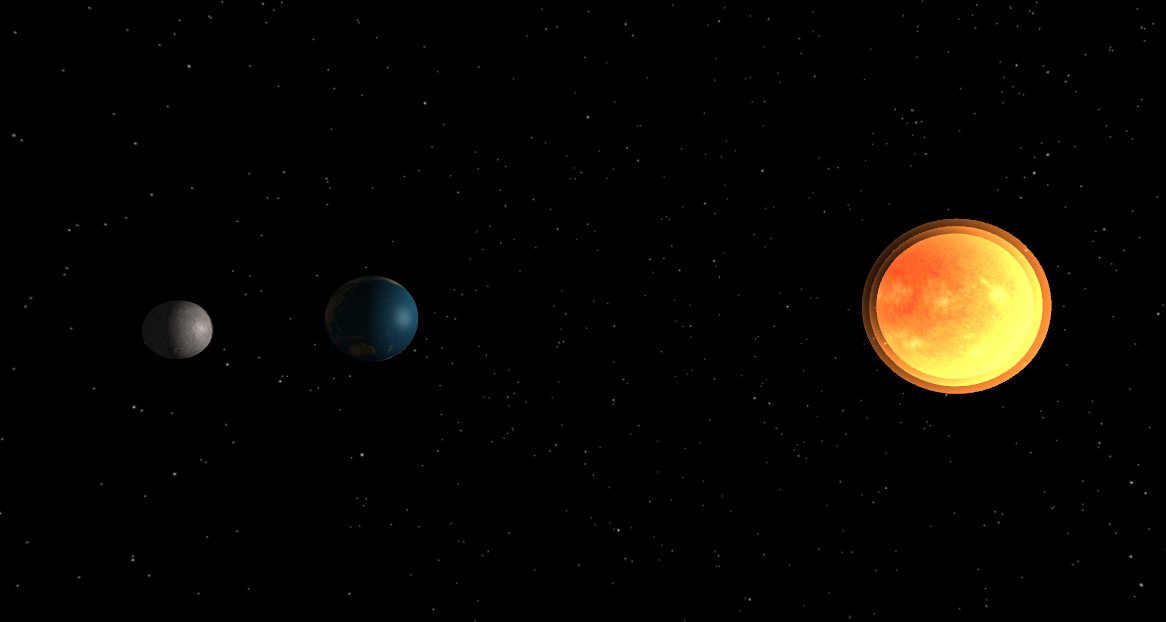
\includegraphics[width=0.5\textwidth]{images/scales}
                \caption{ The Sun, Earth, Moon system after scaling.}
                \label{fig: The Sun, Earth, Moon system after scaling.}
      
\end{figure}

\subsection{Structure}
I have structured my JavaScript code such that there are files for each major component of the model (user interface, Sun-Earth-Moon in one file, Controller, etc) that handles the responsibility of those components, for initiation and updating on each animation loop. For the Sun, Earth and Moon, each is held in their own object, which contains data of their Mesh, a constant reference to their homogeneous coordinates and their update methods.

Most of the parameters for controlling speed, size and the tilts of the planets are contained in a single global variable file, for easy access when I was building and testing my simulation. The setup and main rendering loop are in a single Controller file, and this calls to methods in the other files in the order that things should be initialised and updated. This made it easier to ensure the correct ordering of events.

The Earth and Moon mesh objects have also been added into one single Object3D, earthAndMoon, and then that object has been added to the scene, instead of adding the two individually. This increases the efficiency of the rendering, as they are rendered as one item. While not necessary for such a small simulation, if the application were expanded upon in the future to include many, maybe thousands, of additional planets, this style of structure would be much easier to maintain. It would also help group planets and their moons together, meaning they could be added and removed with their satellites easily.

\subsection{Running the program}
To run the simulation for demonstration, visit: 

\url{http://users.aber.ac.uk/jee22/cs323/virtual-system/}

hosted on my university file store. For building and testing, I ran the application locally using xampp\cite{xampp} . You should be able to see the application in full working order in both B59 and C56, best seen with the Firefox browser. No additional downloading is required. There is also a Credits page for any third party textures and code used in the application here: \url{http://users.aber.ac.uk/jee22/cs323/virtual-system/credits.html}.


%----------------------------------------------------------------------------------------
%	Basic Features
%----------------------------------------------------------------------------------------

\section{Basic Features}
\subsection{The earth orbits the centre of the Sun}
The Earth has a clear orbit around the centre of the Sun, although it is an elliptical orbit and so may look a little off centre in the screenshot. If you view the images below, you can see how the orbit is set up around the Sun. This is achieved through pre-computed points of the orbital rotation using Kepler's 2nd Law of planetary motion (more on this in Additional Features section), which generates an elliptical orbit with varying speeds depending on the point of orbit.

\begin{figure}[H]
        \centering
        \begin{subfigure}[b]{0.4\textwidth}
                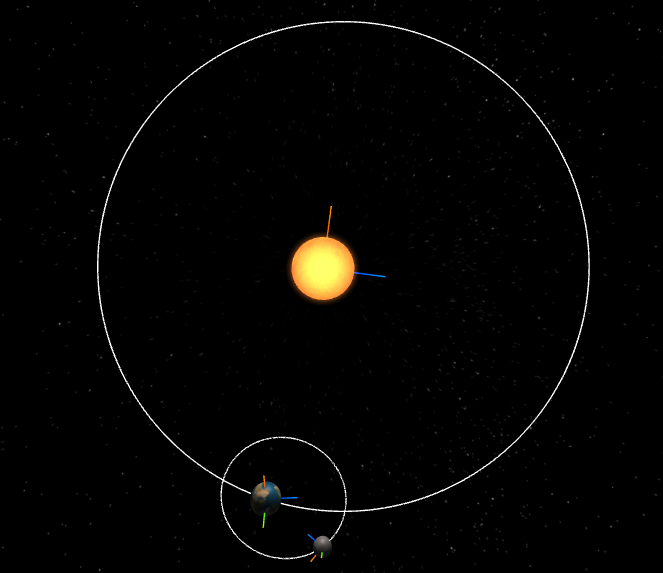
\includegraphics[width=\textwidth]{images/earthorbitsun1}
                \caption{View from above.}
                \label{fig: The Earth orbiting the Sun}
       \end{subfigure}
       %add desired spacing between images, e. g. ~, \quad, \qquad etc.
         %(or a blank line to force the subfigure onto a new line)
        \begin{subfigure}[b]{0.4\textwidth}
                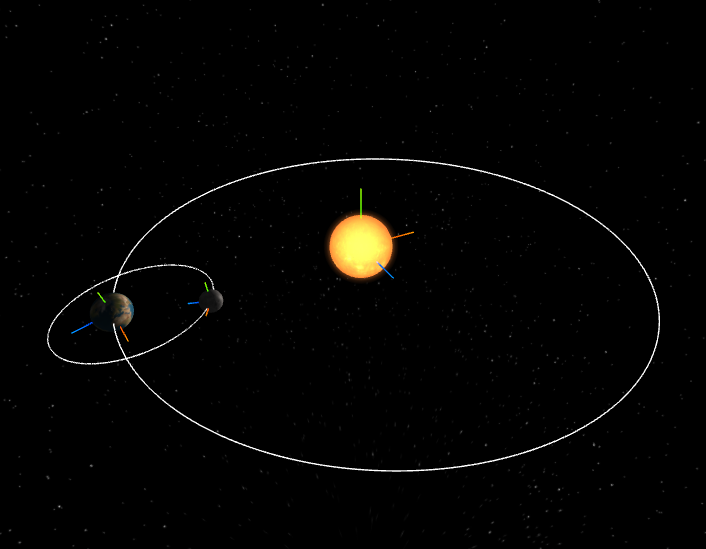
\includegraphics[width=\textwidth]{images/earthorbitsun2}
                \caption{View from the side.}
                \label{fig:The Earth orbiting the Sun}
       \end{subfigure}
       \caption{Views of the Earth's Orbit around the centre of the Sun (elliptical), shown by the orbit lines.}\label{fig: The Earth orbiting the centre of the Sun}
\end{figure}

Originally, the Earth orbited the Sun through updating the x and z coordinates, each animation frame updating the new position of the Earth by shifting it a certain amount, using the distance from the Sun, the speed of rotation the current x and z position and using radians to create the next step on the full anti-clockwise orbit.

\subsection{The moon orbits the centre of the Earth}
The Moon orbits the centre of the Earth in much the same way that the Earth orbits the Sun. The points are precomputed, yet take into account the Earth's current position too. The orbit is elliptical, and as in reality, doesn't sit squarely 'centrally circling' the Earth. More information can be found out about this later in the report.

\begin{figure}[H]
        \centering
        \begin{subfigure}[b]{0.4\textwidth}
                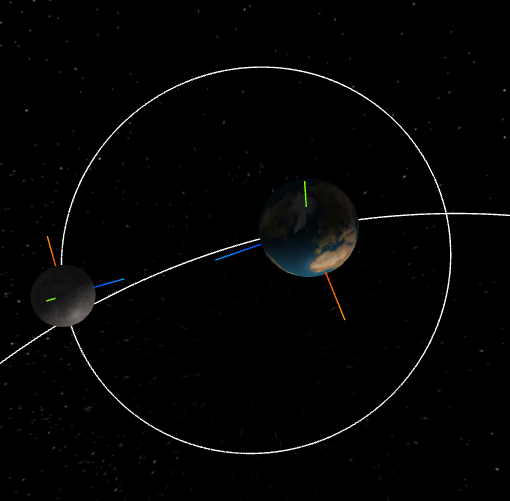
\includegraphics[width=\textwidth]{images/moonorbitearth1}
                \caption{View from above.}
                \label{fig: The Moon orbiting the Earth.}
       \end{subfigure}
       %add desired spacing between images, e. g. ~, \quad, \qquad etc.
         %(or a blank line to force the subfigure onto a new line)
        \begin{subfigure}[b]{0.4\textwidth}
                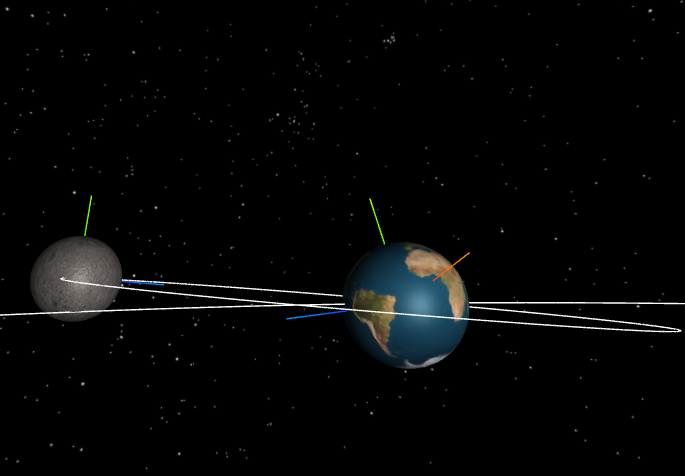
\includegraphics[width=\textwidth]{images/moonorbitearth2}
                \caption{View from the side.}
                \label{fig:The Earth orbiting the Sun}
       \end{subfigure}
       \caption{Views of the Moon's Orbit around the centre of the Earth (elliptical), shown by the orbit lines.}\label{fig: The Moon orbiting the centre of the Earth}
\end{figure}

\subsection{Circular orbits}
When I first built the simulation, the orbits were completely circular, but for a challenge I made them Elliptical, you can see Additional Features for more information. When they were circular though, they were done like this: 

\begin{lstlisting}
function updateOrbit(objectToUpdate, pivotPosition, orbitDistanceFromPivot, orbitAngleThisStep){
     objectToUpdate.position.x = pivotPosition.x + (orbitDistanceFromPivot * -Math.cos(orbitAngleThisStep));
     objectToUpdate.position.z = pivotPosition.z + (orbitDistanceFromPivot * -Math.sin(orbitAngleThisStep));
 }
 \end{lstlisting}
Where objectToUpdate was the Earth or Moon, pivotPosition is the centre of the orbit and point to orbit around, orbitDistanceFromPivot is the distance between the centre of orbit and the object orbiting it and the orbitAngleThisStep being the angle of rotation for the next position for the object to move, in radians.
 
If I were to do this in matrix transformations, I would do a similar process to updating the x and z position, but rather than updating them with .x and .z =, I would turn the coordinates into a homogeneous matrix and then multiply a shift on the x matrix and z matrix transformations together, apply that to the homogeneous coordinates, then convert them back to physical coordinates, update the object's vertices with its new position and then update the face and vertex normals with the normal of the transformation matrix. 
 
Doing this is not necessary for the orbital rotations as they are precomputed. I have, however, done this for axial rotations and this can be seen in the subsection for the Sun, Earth and Moon spinning on their own axes.

\subsection{The Sun, Earth and Moon shown as texture mapped spheres}
As shown below, each object has its own texture mapped to the surface. As an addition to this, the Earth and Moon have bump maps which make it look like their surfaces are not completely smooth, as in reality. The Earth additionally has a specular map, which allows the light from the Phong lighting and shading to reflect off of the reflective water of the Earth but not so much the land masses. The textures for the Earth and Moon come from planetpixel\cite{earthtextures}, while the Sun texture is credited to NASA\cite{suntexture}

\begin{figure}[H]
        \centering
        \begin{subfigure}[b]{0.3\textwidth}
                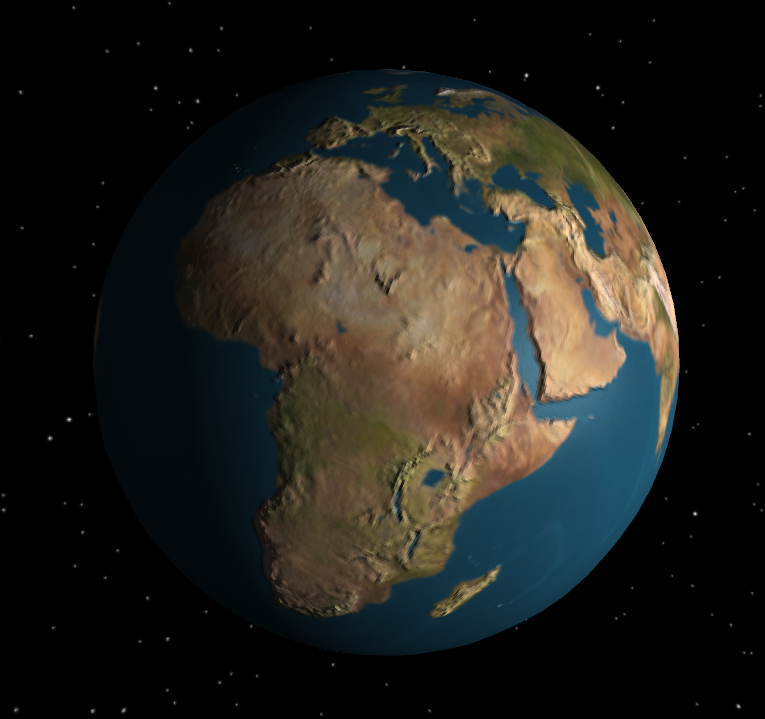
\includegraphics[width=\textwidth]{images/earthtexture}
                \caption{Earth texture maps}
                \label{fig: The Earth texture mapped.}
       \end{subfigure}
       %add desired spacing between images, e. g. ~, \quad, \qquad etc.
         %(or a blank line to force the subfigure onto a new line)
                 \begin{subfigure}[b]{0.3\textwidth}
                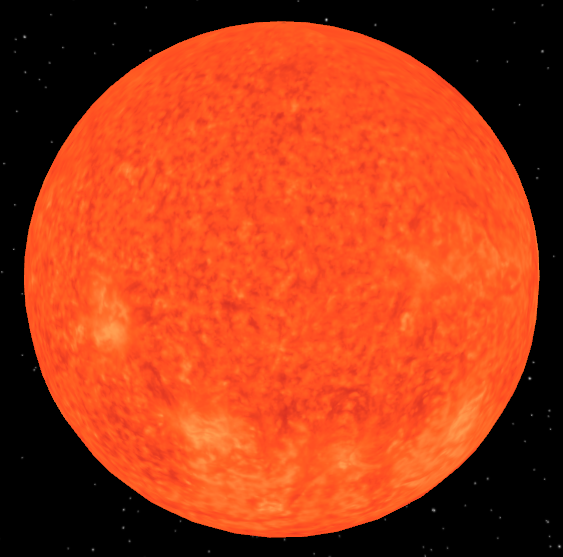
\includegraphics[width=\textwidth]{images/suntexture}
                \caption{Sun texture map}
                \label{fig: The Sun texture mapped}
       \end{subfigure}
        \begin{subfigure}[b]{0.3\textwidth}
                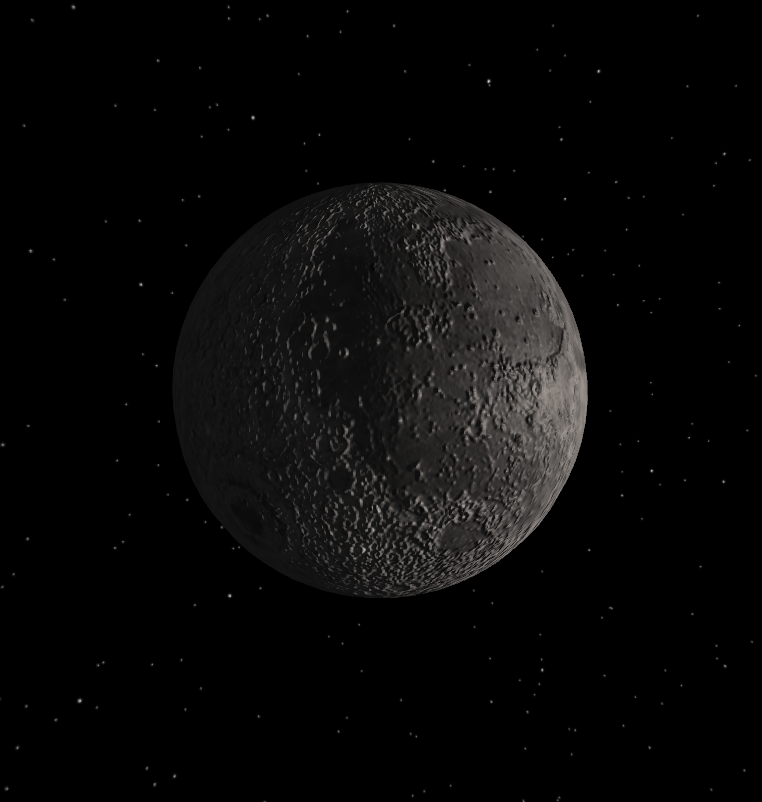
\includegraphics[width=\textwidth]{images/moontexture}
                \caption{Moon texture maps}
                \label{fig: The Moon texture mapped}
       \end{subfigure}
       \caption{The objects of the simulation, texture mapped to look like the planets they represent.}\label{fig: Texture mapped Sun, Earth and Moon.}
\end{figure}

\subsection{The Sun, Earth and Moon each spinning on their own axes}
The Sun, Earth and Moon each spin on their own axis by a rotation on the Y axis. In my first version of the application, this was done through updating the object.rotation.y in increments, based on the objects rotation speed, every animation frame.
\begin{lstlisting}
earthMesh.rotation.y += controlValues.earthAxisRotationSpeed * (Math.PI / 180); // rotate Earth on axis
\end{lstlisting}
This ensured that each planet would rotate (anti-clockwise) based on the global variables provided (combined with the speed of animation via controlValues) and not affect the position or the axial tilt. Later, I changed the process of updating the rotation to using Matrix transformations, and this is covered in Additional Features.

While difficult to show in just images, you can see from figure 5 that the Earth spins on it's own axis.
\begin{figure}[H]
        \centering
        \begin{subfigure}[b]{0.4\textwidth}
                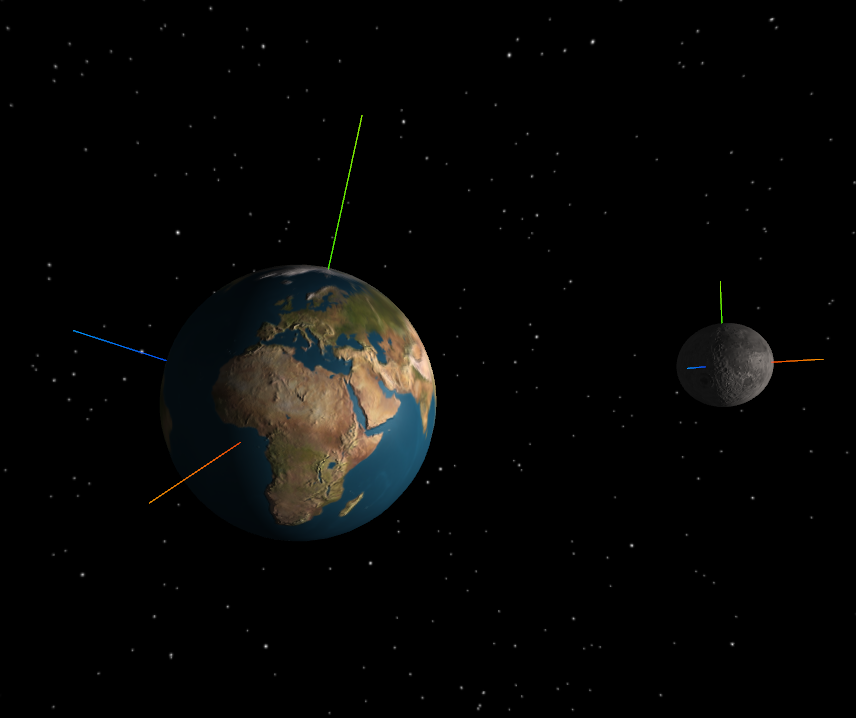
\includegraphics[width=\textwidth]{images/earthandmoonaxisspin1}
                \caption{The Earth spinning on its own axis 1.}
                \label{fig: The axial spin of the Earth 1.}
       \end{subfigure}
        \begin{subfigure}[b]{0.4\textwidth}
                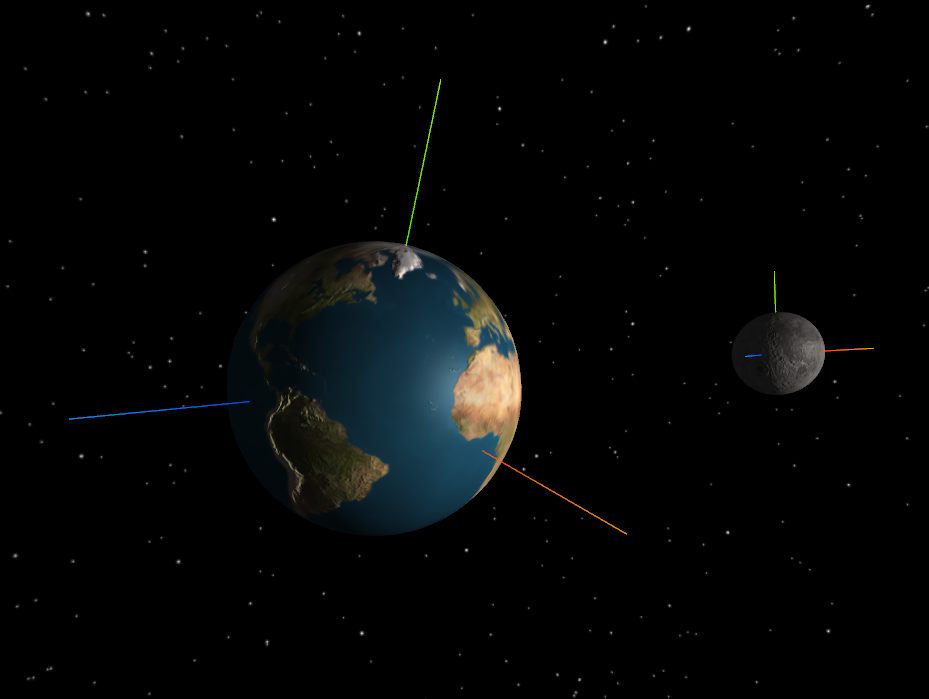
\includegraphics[width=\textwidth]{images/earthandmoonaxisspin2}
                \caption{The Earth spinning on its own axis 2.}
                \label{fig: The axial spin of the Earth 2.}
       \end{subfigure}
               \begin{subfigure}[b]{0.4\textwidth}
                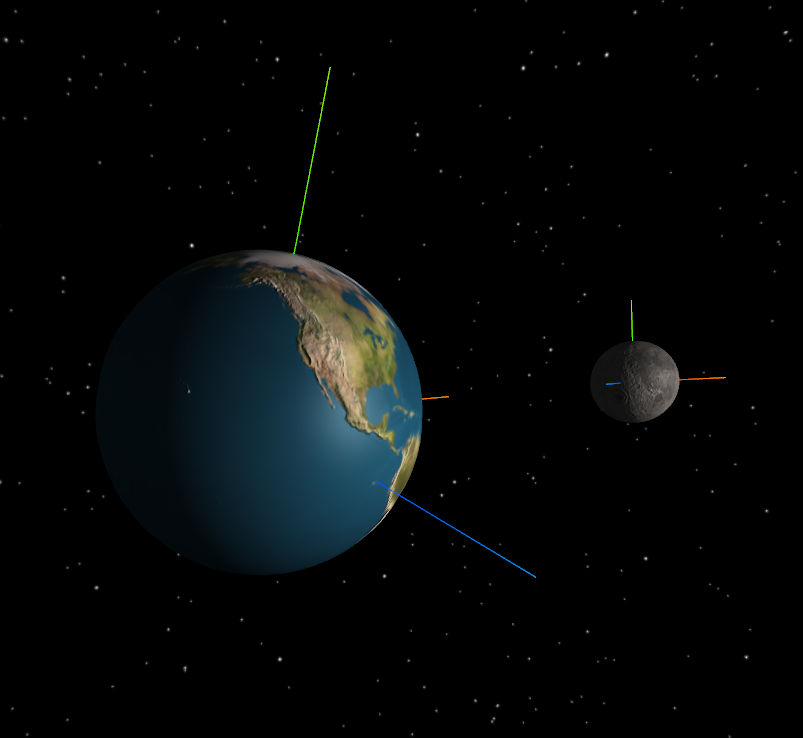
\includegraphics[width=\textwidth]{images/earthandmoonaxisspin3}
                \caption{The Earth spinning on its own axis 3.}
                \label{fig: The axial spin of the Earth 3.}
       \end{subfigure}
               \begin{subfigure}[b]{0.4\textwidth}
                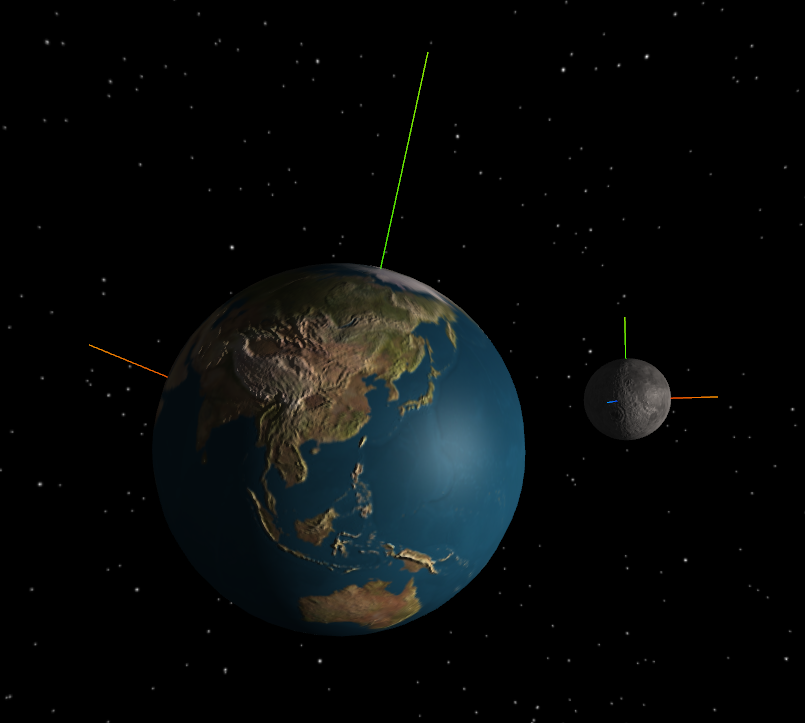
\includegraphics[width=\textwidth]{images/earthandmoonaxisspin4}
                \caption{The Earth spinning on its own axis 4.}
                \label{fig: The axial spin of the Earth 4.}
       \end{subfigure}
       \caption{Collections of images to present the Earth spinning on its own axis.}\label{fig: The Earth's individual rotation.}
\end{figure}

To see the Moon's axial rotation, we can best view it from above, such as with figure 6, showing the full axial rotation (in this case in sync with the orbital rotation around the Earth too. This is covered in more detail in Additional Features).

\begin{figure}[H]
        \centering
        \begin{subfigure}[b]{0.4\textwidth}
                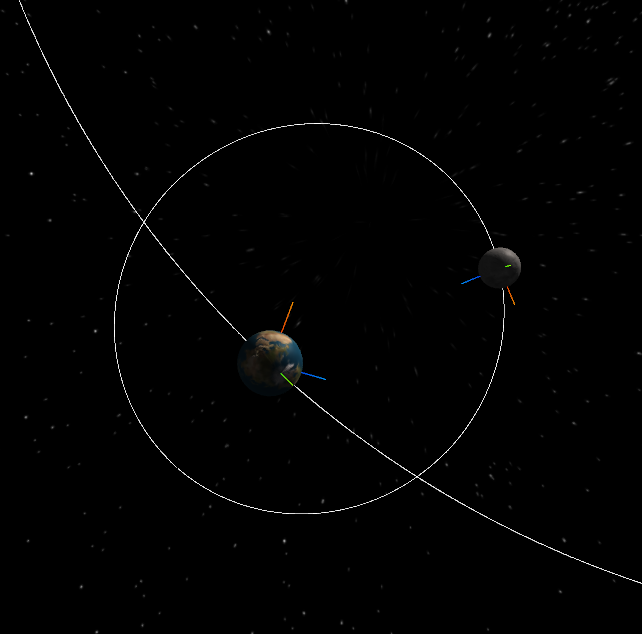
\includegraphics[width=\textwidth]{images/earthandmoonaxisspinabove1}
                \caption{The Moon spinning on its own axis.}
                \label{fig: The axial spin of the Moon.}
       \end{subfigure}
        \begin{subfigure}[b]{0.4\textwidth}
                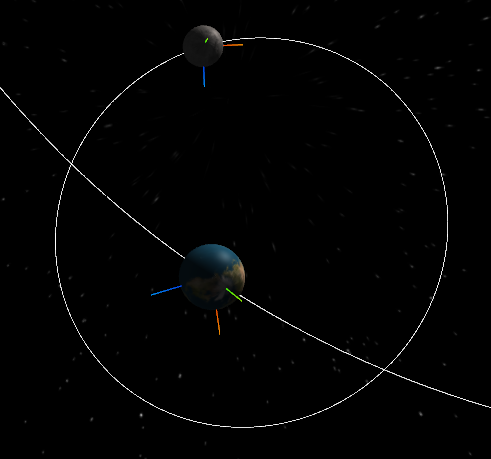
\includegraphics[width=\textwidth]{images/earthandmoonaxisspinabove2}
                \caption{The Moon spinning on its own axis.}
                \label{fig: The axial spin of the Moon.}
       \end{subfigure}
               \begin{subfigure}[b]{0.4\textwidth}
                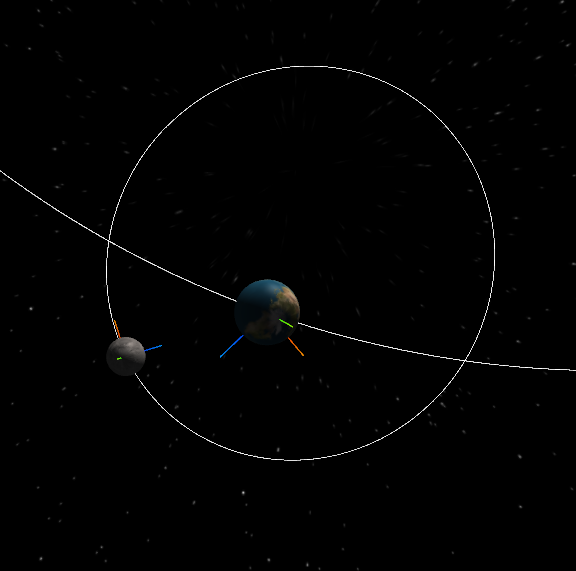
\includegraphics[width=\textwidth]{images/earthandmoonaxisspinabove3}
                \caption{The Moon spinning on its own axis.}
                \label{fig: The axial spin of the Moon.}
       \end{subfigure}
               \begin{subfigure}[b]{0.4\textwidth}
                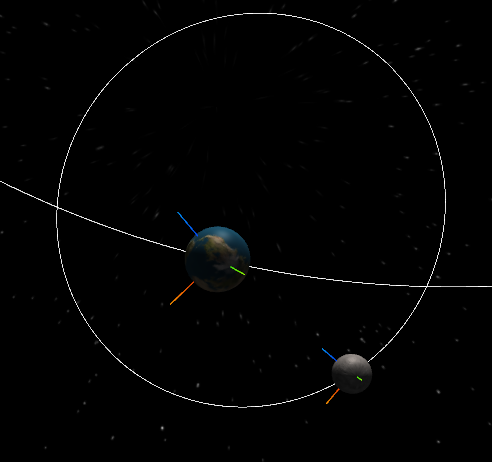
\includegraphics[width=\textwidth]{images/earthandmoonaxisspinabove4}
                \caption{The Moon spinning on its own axis.}
                \label{fig: The axial spin of the Moon.}
       \end{subfigure}
       \caption{Collections of images to present the Moon spinning on its own axis.}\label{fig: The Moon's axial rotation.}
\end{figure}

The Sun also spins on its own axis, as seen in figure 7.

\begin{figure}[H]
        \centering
        \begin{subfigure}[b]{0.4\textwidth}
                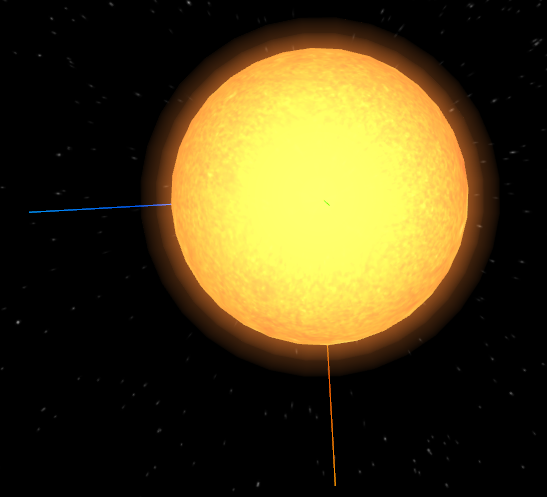
\includegraphics[width=\textwidth]{images/sunaxialrotation1}
                \caption{The Sun spinning on its own axis 1}
                \label{fig: The axial spin of the Sun.}
       \end{subfigure}
        \begin{subfigure}[b]{0.4\textwidth}
                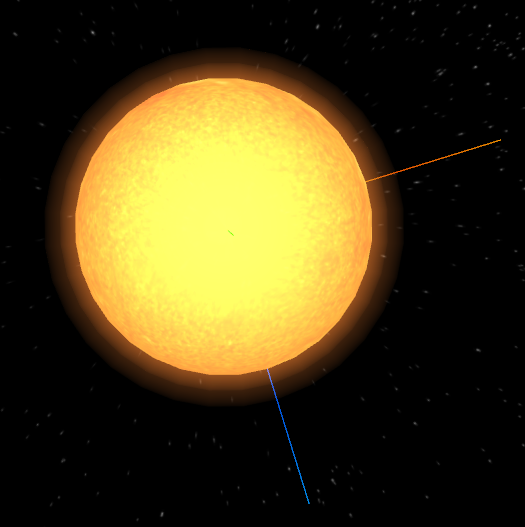
\includegraphics[width=\textwidth]{images/sunaxialrotation2}
                \caption{The Sun spinning on its own axis 2}
                \label{fig: The axial spin of the Sun.}
       \end{subfigure}
               \begin{subfigure}[b]{0.4\textwidth}
                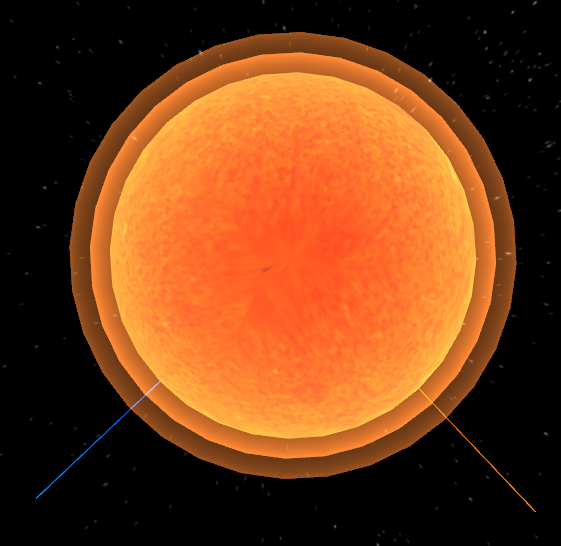
\includegraphics[width=\textwidth]{images/sunaxialrotation3}
                \caption{The Sun spinning on its own axis 3}
                \label{fig: The axial spin of the Sun.}
       \end{subfigure}
       \caption{Collections of images to present the Sun spinning on its own axis.}\label{fig: The Sun's axial rotation.}
\end{figure}

\subsection{The sun shown as a self-illuminated sphere}
To present the Sun as a self-illuminated sphere, I first used an emissive map, which lights the texture applied to the Mesh, and then added some Ambient lighting, for the purpose of showing the Sun as if it had it's own light and also to help the viewer see the backs of the planets too. Additionally, I thought it looked good to have a glowing effect around the Sun. I achieved this using the technique by Lee Stemkoski\cite{sunglow}. I created two glow effects, one larger than the other, to give the impression of the light being more intense as the viewer looked directly at the Sun. 

\begin{figure}[H]
        \centering
        \begin{subfigure}[b]{0.4\textwidth}
                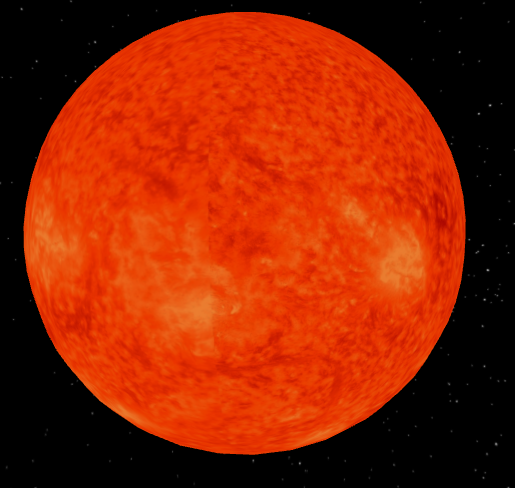
\includegraphics[width=\textwidth]{images/sunemissive}
                \caption{The Sun with just an emissive map for self-illuminating}
                \label{fig:Self-illuminating Sun with emissive map.}
       \end{subfigure}
       %add desired spacing between images, e. g. ~, \quad, \qquad etc.
         %(or a blank line to force the subfigure onto a new line)
        \begin{subfigure}[b]{0.4\textwidth}
                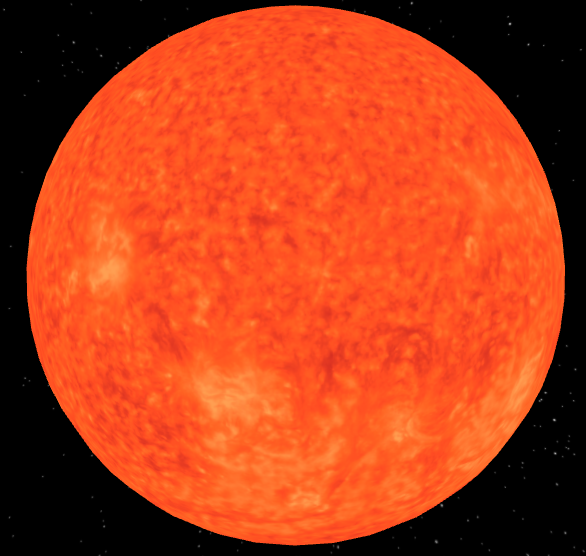
\includegraphics[width=\textwidth]{images/sunemissiveandambient}
                \caption{The Sun with emissive map and ambient lighting.}
                \label{fig:Self-illuminating Sun with emissive map.}
       \end{subfigure}
        \begin{subfigure}[b]{0.4\textwidth}
                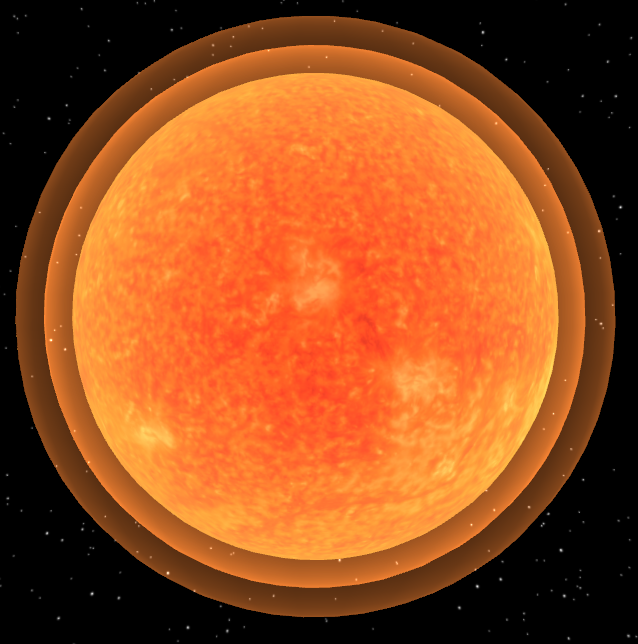
\includegraphics[width=\textwidth]{images/sunwithglow}
                \caption{The Sun with emissive map, ambient lighting and glow effect.}
                \label{fig:Self-illuminating Sun with emissive map.}
       \end{subfigure}
        \caption{The Sun with the three ways it is presented as self-illuminated.}\label{fig:Self-illuminated Sun}
\end{figure}

\subsection{Earth and Moon lit by a single point light source located at the centre of the Sun}
All objects in the scene are lit slightly by a dark AmbientLight for the purpose of the animation. The light source from the Sun is a SpotLight, not a PointLight as requested by the Basic Features. The main reason for this is that Point Lights in three.js do not cast shadows (note: As of writing this, PointLights may now cast shadows, or at least a solution for this is being made. For the sake of computation costs, I have stuck with using a SpotLight). 

In order to light the Earth and Moon with the Spot Light, I have the light starting at the centre of the Sun (0,0,0) and added as part of the SunMesh for rendering efficiency, and its target set as the position of the Earth, tracking it every animation frame to give the illusion of a single light source at the centre of the Sun.

\begin{lstlisting}
function buildSunLight(){
  var ambientLight = new THREE.AmbientLight(0x222222);
  scene.add(ambientLight);

  sunLight = new THREE.SpotLight(0xfff0e6, 1, 0);
  sunLight.castShadow = true;

  sunLight.target = earthMesh;    
  sunLight.position.set(sunMesh.position.x, sunMesh.position.y, sunMesh.position.z);
  sunMesh.add(sunLight);
}
\end{lstlisting}

%----------------------------------------------------------------------------------------
%	Additional Features
%----------------------------------------------------------------------------------------

\section{Additional Features}
\subsection{User Interface}
To help the user control and view the simulation, I added a number of user interface controls. Using the sidebar interface, a user can change the animation speed, change the camera focus to look at the Sun, Earth or Moon, reset the camera, pause the simulation (pauses the updating of values while still rendering the scene) and turn on or off helpers to visually see the orbital rotations and the axes of the objects. The side bar user interface is made using dat.gui\cite{datgui}, which makes for quick and easy gui by adding controls and parameters for them, including values and functions.

\begin{figure}[H]
        \centering
        \begin{subfigure}[b]{0.4\textwidth}
                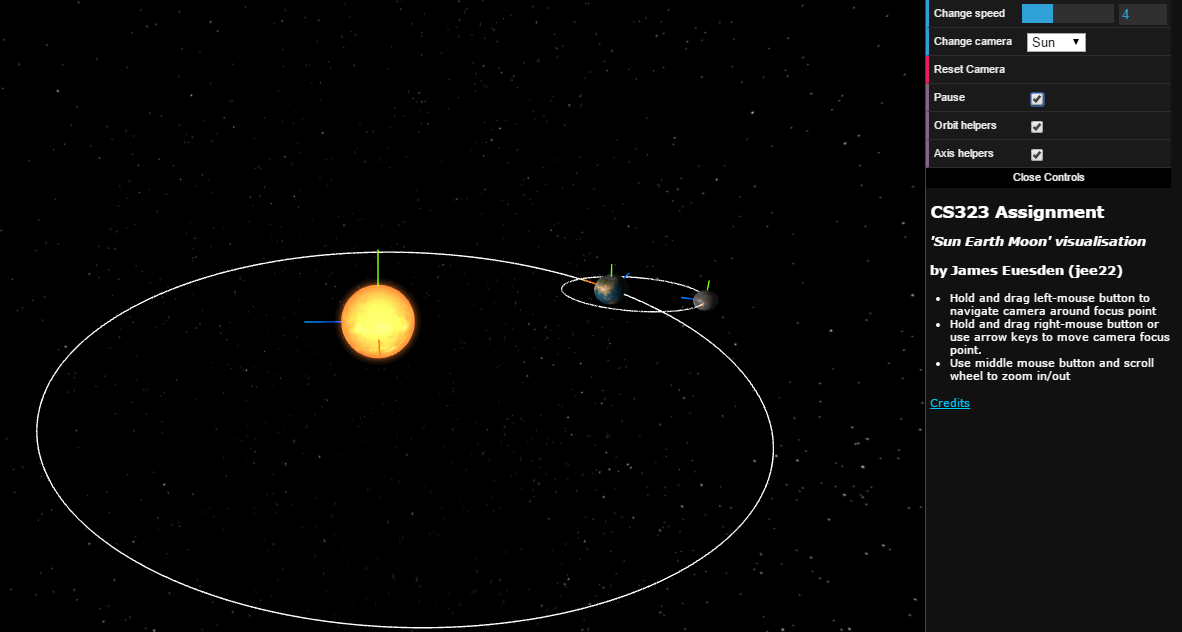
\includegraphics[width=\textwidth]{images/userinterface}
                \caption{The user interface on the page.}
                \label{fig: The user interface.}
	 \end{subfigure}
        \begin{subfigure}[b]{0.4\textwidth}
                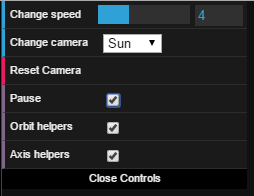
\includegraphics[width=\textwidth]{images/closeupui}
                \caption{The user interface up close.}
                \label{fig: Close up of the user interface.}
	 \end{subfigure}
\end{figure}

\begin{lstlisting}
var params = {
    "speed": 1,
    "cameraFocus": 0,
    "resetCamera" : resetCamera,
    "pause": false,
    "orbitHelpers": true,
    "axisHelpers": true
};

function setupGUI() {
    var gui = new dat.GUI();
    gui.add( params, "speed" ).min(1).max(10).step(1).name('Change speed').onChange( function( value ) {
        updateControlValues(value);
    } );

    gui.add( params, 'cameraFocus', {Sun: 0, Earth: 1, Moon: 2} ).name('Change camera focus').onChange( function(value) {
      if(value == 0){
        controls.target = sunMesh.position;
      } else if(value == 1){
        controls.target = earthMesh.position;
      } else if(value == 2){
        controls.target = moonMesh.position;
      }
    });

    gui.add(params, 'resetCamera').name('Reset Camera');

    gui.add(params, 'pause').name('Pause').onChange( function( value ){
        simulationPaused = value;
    });
    
    gui.add(params, 'orbitHelpers').onChange( function( value ){
        earthOrbitLine.visible = value;
        moonOrbitLine.visible = value;
    }).name('Orbit helpers');

    gui.add(params, 'axisHelpers').onChange( function( value ){
        earthAxisHelper.visible = value;
        moonAxisHelper.visible = value;
        sunAxisHelper.visible = value;
    }).name('Axis helpers');    
}
\end{lstlisting}

The user can also navigate around the simulation using their mouse or the arrow keys using OrbitControls\cite{orbitcontrols}.

\subsection{Synchronous orbital and axial rotation of the Moon}
By using the same speed for the Moon's orbital and axial rotation in the simulation, the Moon can be set so that the same face is always shown to the Earth. When I was updating the Moon's orbit by computing the next step every animation frame, I would use the same speed value for both the rotation update and orbit update. However, since I change to precomputing the elliptical orbit, the speeds no longer had a way to match up.

One option I could take is to continue computing the axial rotation every animation step, but only as often as I update the orbital rotation step, to ensure they stayed in sync. However, doing this, plus with the Moon's rotation being titled, requires a fair amount of computation to try and get the synchronisation correct. In order to save time on coding and avoid a `wobbly' Moon, I used the three.js function 
\begin{lstlisting}
  moonMesh.lookAt(earthMesh.position);\end{lstlisting}
 every animation frame. This keeps the synchronous axial and orbital rotation around the Earth.
 
 \begin{figure}[H]
        \centering
        \begin{subfigure}[b]{0.38\textwidth}
                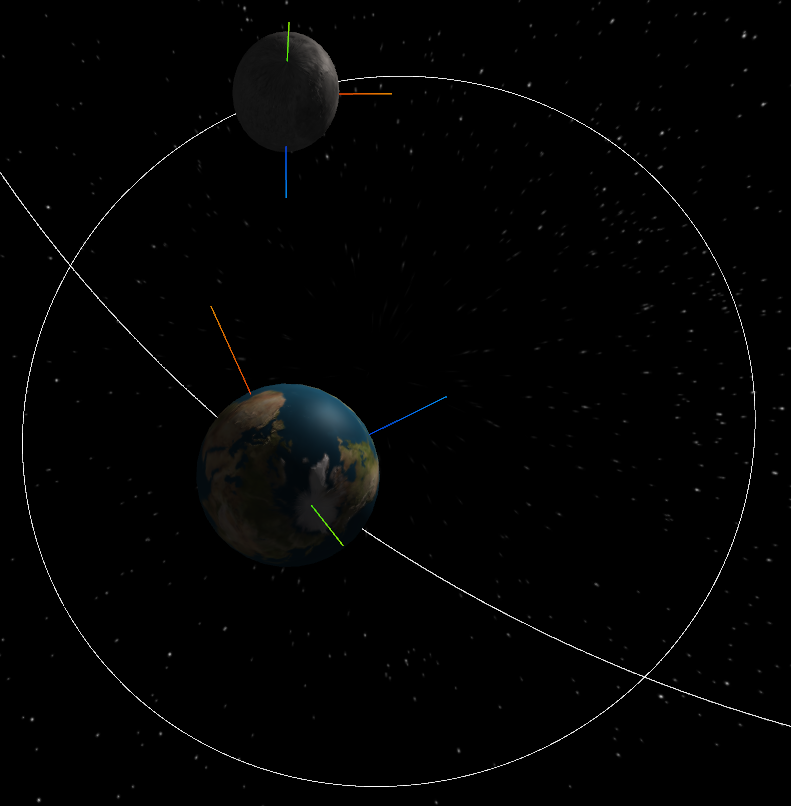
\includegraphics[width=\textwidth]{images/syncrotation1}
                \caption{Synchronous axial and orbital rotation of the Moon 1.}
                \label{fig: Synchronous axial and orbital rotation of the Moon.}
	 \end{subfigure}
        \begin{subfigure}[b]{0.38\textwidth}
                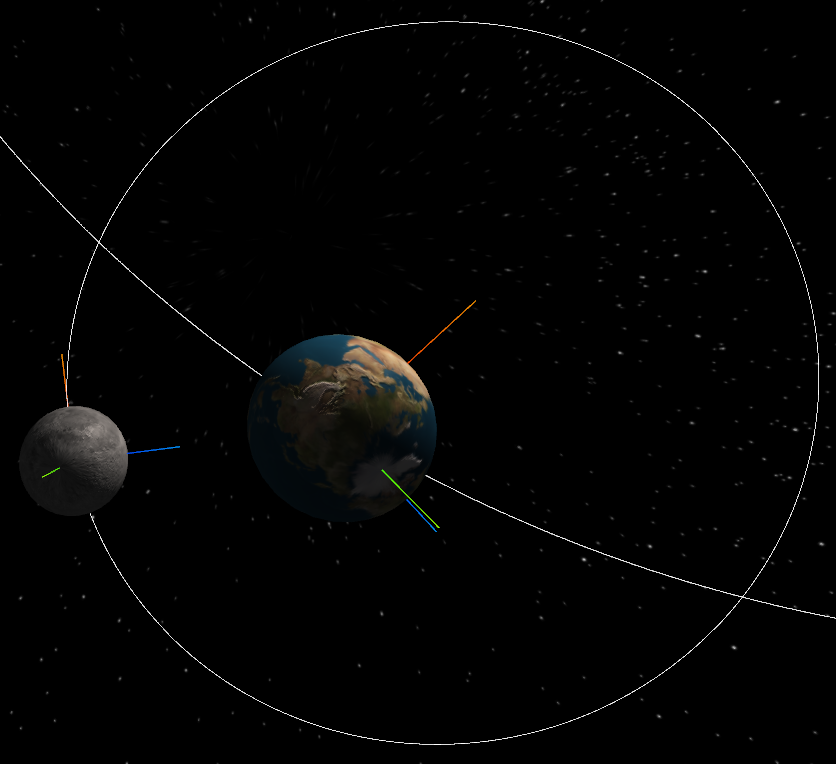
\includegraphics[width=\textwidth]{images/syncrotation2}
                \caption{Synchronous axial and orbital rotation of the Moon 2.}
                \label{fig: Synchronous axial and orbital rotation of the Moon.}
	 \end{subfigure}
	 \begin{subfigure}[b]{0.38\textwidth}
                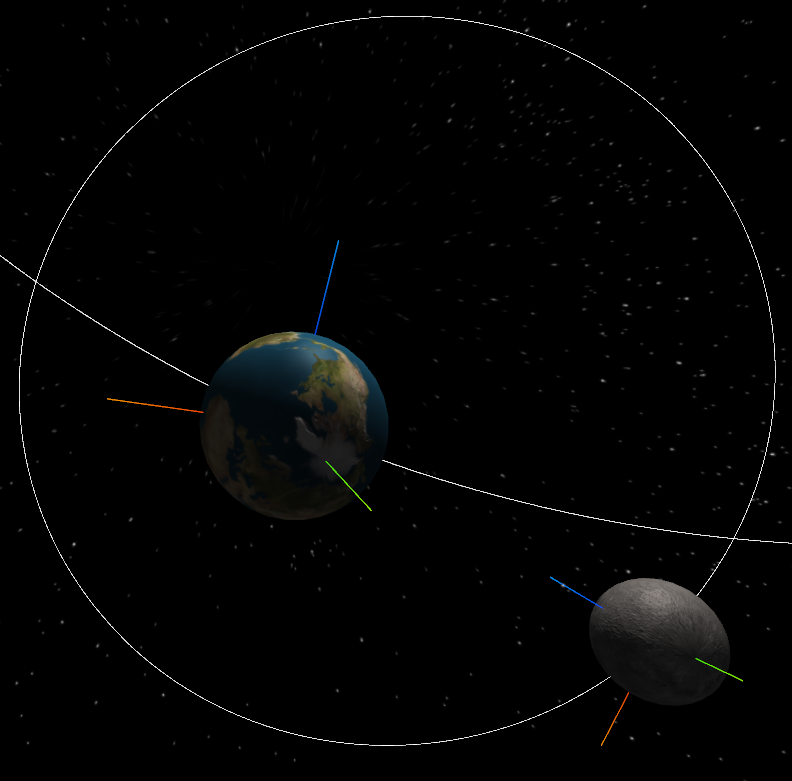
\includegraphics[width=\textwidth]{images/syncrotation3}
                \caption{Synchronous axial and orbital rotation of the Moon 3.}
                \label{fig: Synchronous axial and orbital rotation of the Moon.}
	 \end{subfigure}
	 \caption{You can see the blue axial line, always pointing out from the same face, is always pointing at the Earth.}
\end{figure}

\subsection{Lighting of the Earth and Moon in Phong shading \& Non-illuminated parts of the Earth and Moon to be shown in shadow}
The Materials of the Earth and Moon are made from PhongMaterial, and so Phong lighting and shading is applied through this. Through using Phong shading I was able to better represent how the system looks in reality, with the parts of the Earth and Moon not in the light shown in shadow, and those in the light being brighter.

 \begin{figure}[H]
        \centering
        \begin{subfigure}[b]{0.4\textwidth}
                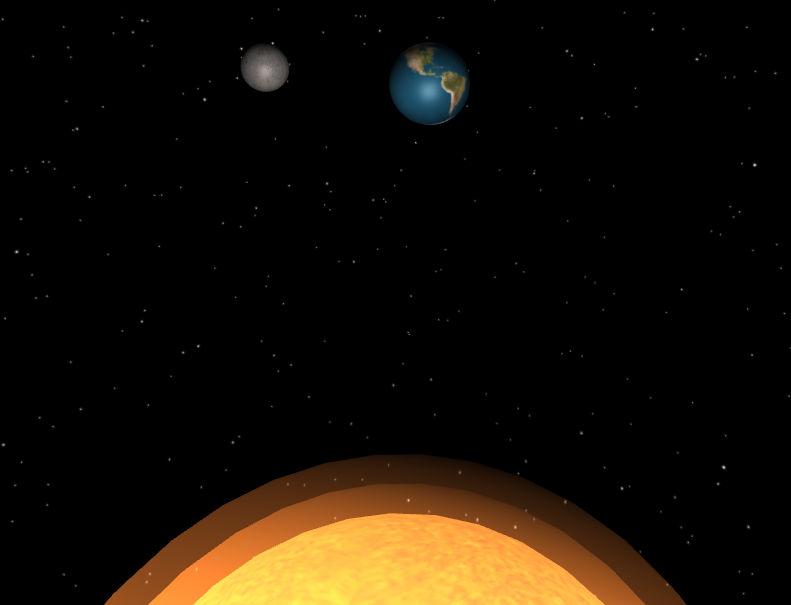
\includegraphics[width=\textwidth]{images/lightfromphong1}
                \caption{Light from the SpotLight on the PhongMaterial.}
                \label{fig: Light from the SpotLight on the PhongMaterial.}
	 \end{subfigure}
        \begin{subfigure}[b]{0.4\textwidth}
                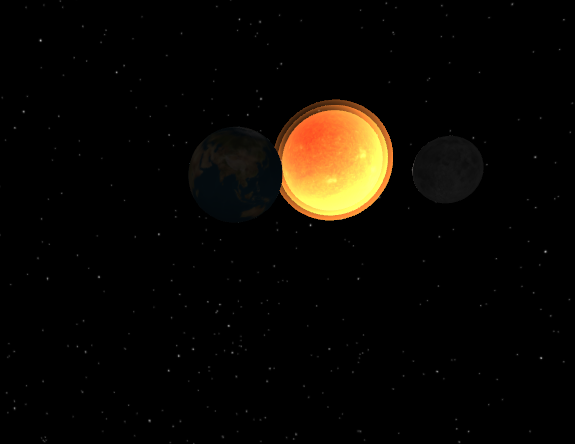
\includegraphics[width=\textwidth]{images/lightfromphong2}
                \caption{Shadows from the absence of light from SpotLight on the PhongMaterial.}
                \label{fig: Shadows from the absence of light from SpotLight on the PhongMateria.}
	 \end{subfigure}
	 \caption{The effect of light on the PhongMaterial causing Phong shading.}
\end{figure}

In particular, where I have used a specular map for the Earth's ocean, you can see the shiny light reflection. During my testing, I changed the value of the shininess of the Earth to see how it would look, which can be seen in figure 12.

 \begin{figure}[H]
        \centering
        \begin{subfigure}[b]{0.25\textwidth}
                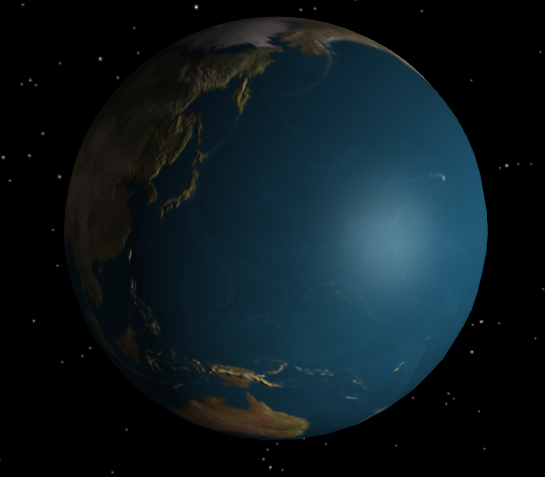
\includegraphics[width=\textwidth]{images/specular1}
                \caption{Specular Lighting.}
                \label{fig:Specular 1.}
	 \end{subfigure}
        \begin{subfigure}[b]{0.25\textwidth}
                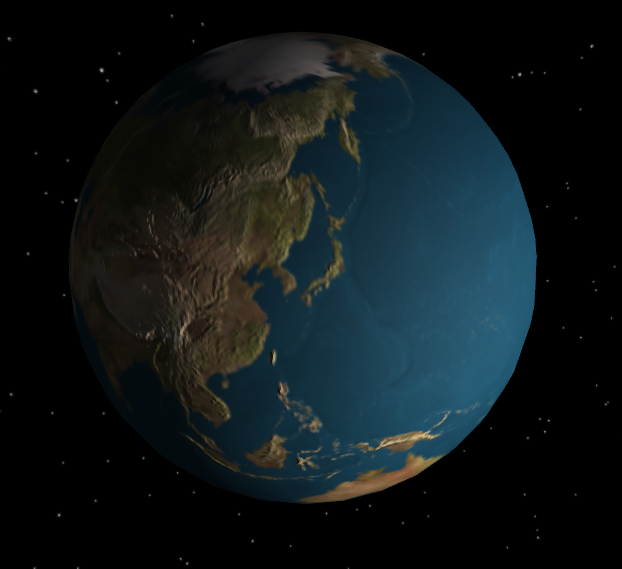
\includegraphics[width=\textwidth]{images/specular2}
                \caption{With no shininess.}
                \label{fig:Specular 2.}
	 \end{subfigure}
	         \begin{subfigure}[b]{0.25\textwidth}
                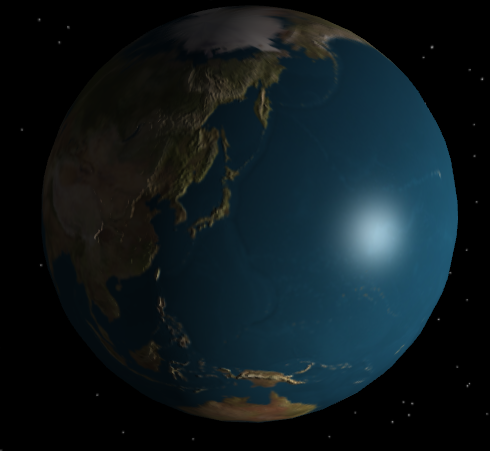
\includegraphics[width=\textwidth]{images/specular3}
                \caption{High shininess.}
                \label{fig:Specular 3.}
	 \end{subfigure}
	         \begin{subfigure}[b]{0.25\textwidth}
                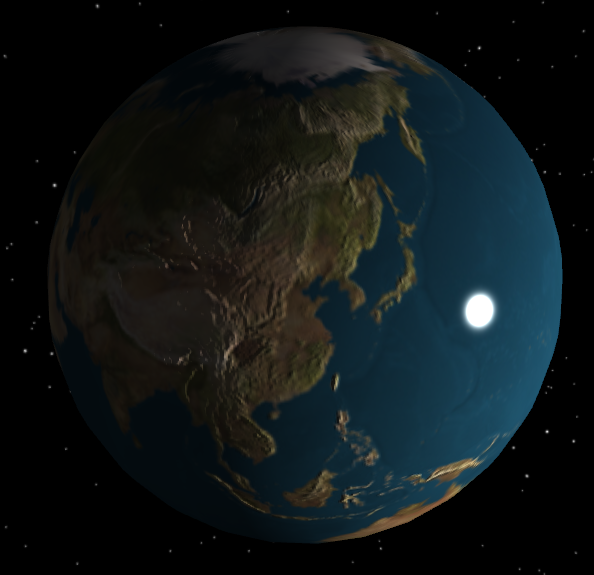
\includegraphics[width=\textwidth]{images/specular4}
                \caption{Maximum shininess.}
                \label{fig:Specular 4.}
	 \end{subfigure}
	         \begin{subfigure}[b]{0.25\textwidth}
                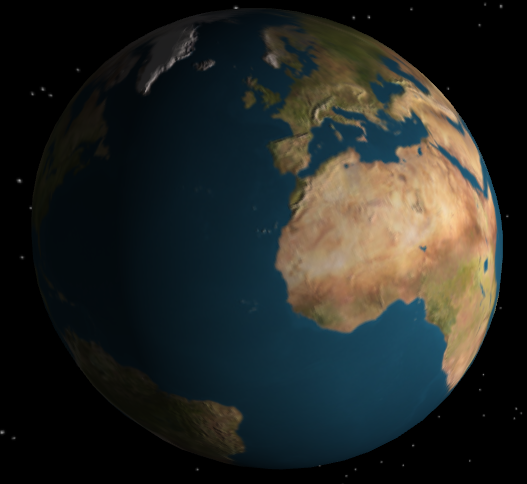
\includegraphics[width=\textwidth]{images/specular5}
                \caption{The landmasses do no reflect the light as much.}
                \label{fig:Specular 5.}
	 \end{subfigure}
	 \caption{Testing what happens when the shininess is turned up on the Phong material with a specular map.}
\end{figure}

As an effect of using a SpotLight and Phong Material, the sides facing away from the Sun are non-illuminated, and so shown in shadow, no matter where the objects are in relation to the Sun (and so the light), the opposite side is in shadow. There is still Ambient Light to display some detail of the shadow sections, but otherwise they are shown to be dark. This happens automatically when using any light that has a direction (Spot, Directional, Point, but not Ambient) and Phong (or Lambert) material.

 \begin{figure}[H]
        \centering
        \begin{subfigure}[b]{0.4\textwidth}
                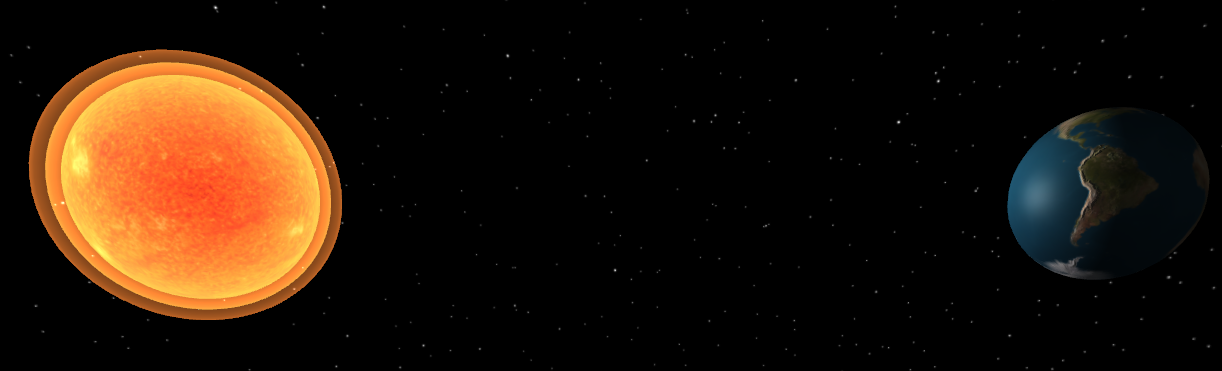
\includegraphics[width=\textwidth]{images/lightfromphong3}
                \caption{The side of the Earth facing the Sun is bright, while the side not illuminated is in shadow.}
                \label{fig: The side of the Earth facing the Sun is bright, while the side not illuminated is in shadow.}
	 \end{subfigure}
        \begin{subfigure}[b]{0.4\textwidth}
                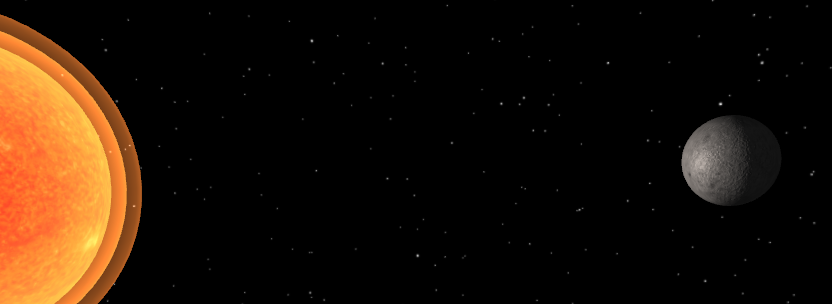
\includegraphics[width=\textwidth]{images/lightfromphong4}
                \caption{The side of the Moon facing the Sun is bright, while the side not illuminated is in shadow.}
                \label{fig: The side of the Moon facing the Sun is bright, while the side not illuminated is in shadow.}
	 \end{subfigure}
	 \caption{The non-illuminated sides of the Earth and Moon are shown in shadow.}
\end{figure}

\subsection{Constant tilt of the Earth's axis}
With the aid of Axis Helper, we can see that the Earth's axis is constantly tilted by 23.44. No matter where it is on it's orbital rotation, the Earth is always tilted in the same direction, simulating the reality of the earth being `flung' around the Sun by the orbit, not turned with it.

 \begin{figure}[H]
        \centering
        \begin{subfigure}[b]{0.6\textwidth}
                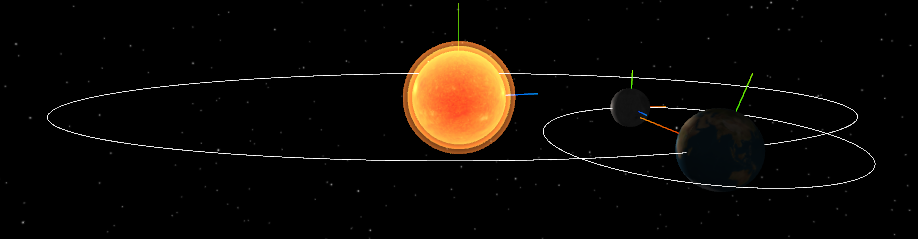
\includegraphics[width=\textwidth]{images/earthtilt1}
                \label{fig: Earth tilt1.}
	 \end{subfigure}
        \begin{subfigure}[b]{0.6\textwidth}
                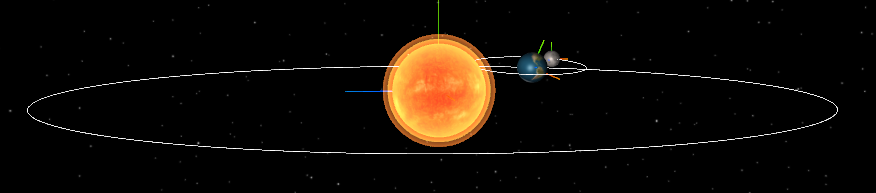
\includegraphics[width=\textwidth]{images/earthtilt2}
                \label{fig: Earth tilt2.}
	 \end{subfigure}
	         \begin{subfigure}[b]{0.6\textwidth}
                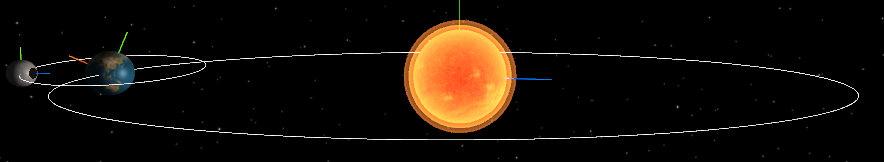
\includegraphics[width=\textwidth]{images/earthtilt3}
                \label{fig: Earth tilt3.}
	 \end{subfigure}
	 \caption{The Earth is tilted the same direction and angle at each point during its orbit, shown by the green line of the Axis Helper.}
\end{figure}

This is super simple to achieve. We just set the Earth's rotation on the z axis to be 23.4 once, when we create it, and then it will always be tilted in that direction, no matter where it is or how the axial rotation on the y axis or orbital rotation and Earth position changes.

\begin{lstlisting}
  earthMesh.rotation.x = (earthAxialTilt/180)*Math.PI;
  earthAxisHelper = new THREE.AxisHelper( earthSize * 2 );
  earthAxisHelper.visible = true;
  earthMesh.add( earthAxisHelper );
\end{lstlisting}

\subsection{Constant tilt of the Moon's orbit}

The Moon's orbit is always tilted, no matter where the Earth is, the orbit is tilted following the Earth, and doesn't wobble. To tilt the orbital rotation of the moon, when the pre-computed points of orbit are computed, they are then multiplied by a rotation on the z axis with a transformation matrix. I chose to use three.js applyMatrix4 with my own rotation matrix.

\begin{lstlisting}
var rotationYMatrix4 = function (angle) {     
        tempMatrix4.set(
            Math.cos(angle), 0, Math.sin(angle), 0,
            0,1,0,0,
            -Math.sin(angle), 0, Math.cos(angle), 0,
            0,0,0,1
            );
        return tempMatrix4;
}

var moonOrbitPoints = calculateOrbitalPoints(orbitSteps, moonOrbitEccentricity, moonDistanceFromEarth);
for(var i = 0; i < moonOrbitPoints.length; i++){
  moonOrbitPoints[i].applyMatrix4(rotationZMatrix4(-(moonOrbitalTilt * (Math.PI / 180))));
}
\end{lstlisting}

This constant tilt can be seen in Figure 15.

\begin{figure}[H]
 \centering
        \begin{subfigure}[b]{0.9\textwidth}
                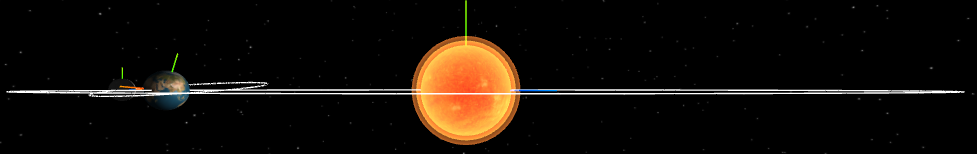
\includegraphics[width=\textwidth]{images/moonorbitaltilt1}
                \label{fig: Moon orbital tilt 1.}
	 \end{subfigure}
        \begin{subfigure}[b]{0.9\textwidth}
                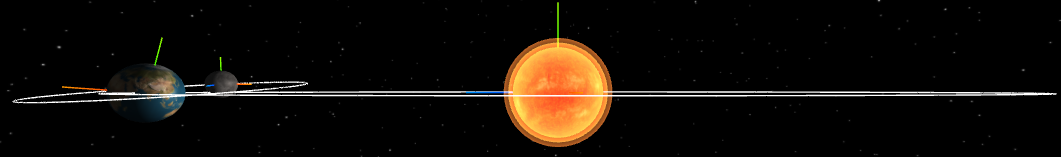
\includegraphics[width=\textwidth]{images/moonorbitaltilt2}
                \label{fig: Moon orbital tilt 2.}
	 \end{subfigure}
	  \begin{subfigure}[b]{0.9\textwidth}
                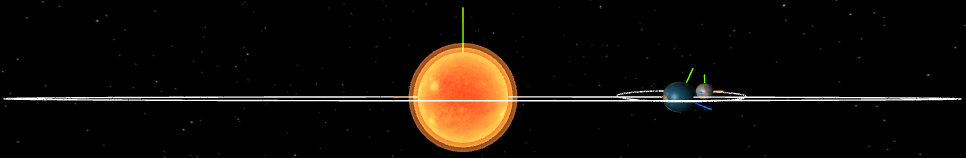
\includegraphics[width=\textwidth]{images/moonorbitaltilt3}
                \label{fig: Moon orbital tilt 3.}
	 \end{subfigure}
	 \caption{The constant orbital tilt of the Moon.}
\end{figure}

\subsection{Elliptical Orbits \& Non-uniform orbital velocities: Kepler's 2nd Law of Planetary Motion}
The calculating of the elliptical orbits and using Kepler's 2nd Law of Planetary Motion tie together, in that when calculating Kepler's 2nd Law we also get the points for an elliptical orbit. I used the formula provided in the assignment brief \cite{assignment} in order to achieve this, and my code can be seen here:
\begin{lstlisting}
// Kepler's 2nd Law calculations (for all points along an orbital rotation, in n (timeStep) steps).
function calculateOrbitalPoints(timeStep, eccentricity, semiMajorAxis){
	 // 2 * Pi is radians for 360 circle;
	var completeCircle = Math.PI * 2;
	var theta = 0;
	var r;
	var orbitPoints = [];
	// +1 to ensure a complete circle with no gaps.
	while(theta <= completeCircle){
		theta += calculateTheta(timeStep, eccentricity, theta);
		r = calculateR(semiMajorAxis, eccentricity, theta);
		orbitPoints.push(new THREE.Vector3(r * -Math.cos(theta), 0, r * Math.sin(theta)));
	}
	return orbitPoints;
}

function calculateTheta(timeStep, eccentricity, theta){
	return (2 / timeStep) * Math.pow((1 + eccentricity * Math.cos(theta)), 2) / Math.pow((1 - Math.pow(eccentricity), 2), (3 / 2));
}

function calculateR(semiMajorAxis, eccentricity, theta){
	var r = (semiMajorAxis * (1 - Math.pow(eccentricity, 2)) / (1 + eccentricity * Math.cos(theta)));
	return r;
}
\end{lstlisting}

To use the function, the points are calculated by providing a timeStep (this is the orbital period of the rotation, e.g. 365 for Earth, and just means how many steps there will be for a complete orbit from starting point to end), the orbit eccentricity and the semi-major axis of the objects rotation, which is the maximum distance of the orbit of the pivot point to the object rotating around it. Once the points have been made, every time the update function is called during the animation loop, the object moves to the next point of orbit, based on the speed of animation.

\begin{lstlisting}
var earthOrbitPoints = calculateOrbitalPoints(earthOrbitalPeriod, earthOrbitEccentricity, earthDistanceFromSun);

updateEarth : function(){
    earthStep+= speed;
    if(earthStep >= earthOrbitPoints.length){
      earthStep = 0;
    }
    var currentPosition = earthOrbitPoints[Math.floor(earthStep)];
    earthMesh.position.set(currentPosition.x, currentPosition.y, currentPosition.z);
}
\end{lstlisting}
You can see the results of the orbital point calculations in figure 16. By changing the eccentricity, we can change the size of the ellipse, and in effect the speed of the object in its orbit as it reaches points closer to the object it is orbiting around.

 \begin{figure}[H]
        \centering
        \begin{subfigure}[b]{0.4\textwidth}
                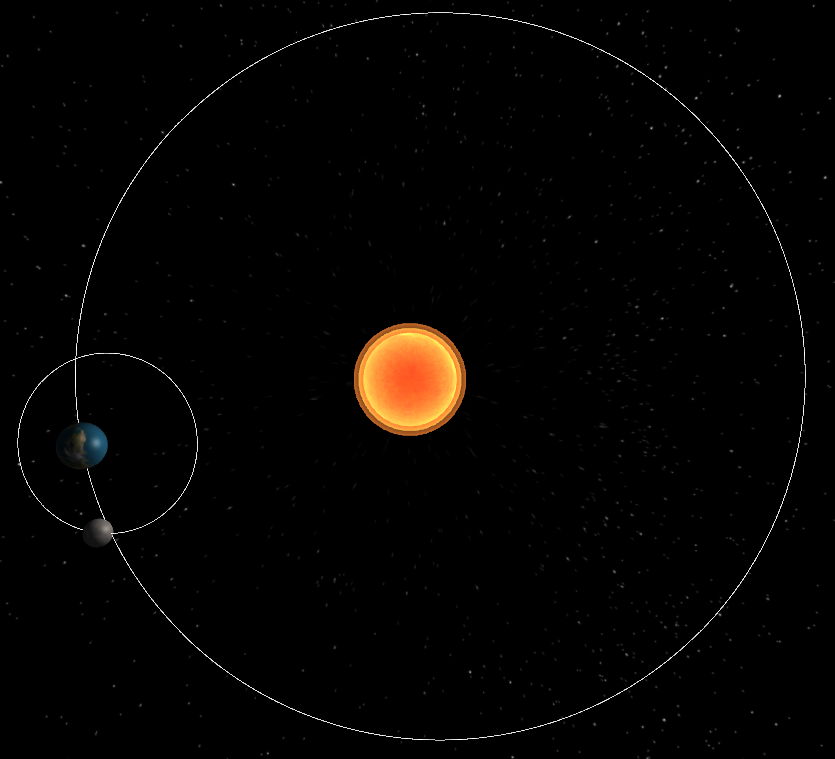
\includegraphics[width=\textwidth]{images/earthelliptical}
                \caption{Earth's elliptical orbit.}
                \label{fig: Earth's elliptical orbit.}
	 \end{subfigure}
        \begin{subfigure}[b]{0.4\textwidth}
                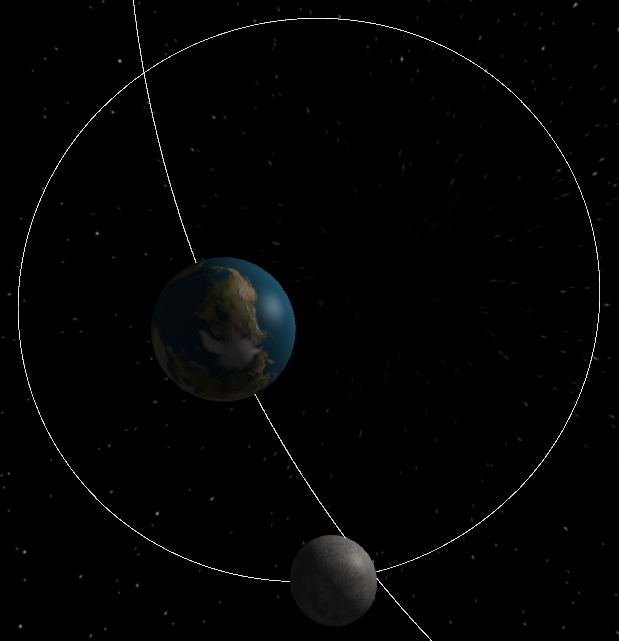
\includegraphics[width=\textwidth]{images/moonelliptical}
                \caption{Moon's elliptical orbit.}
                \label{fig: Moon's elliptical orbit.}
	 \end{subfigure}
        \begin{subfigure}[b]{0.54\textwidth}
                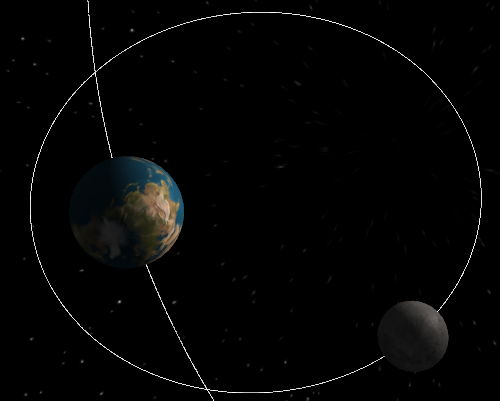
\includegraphics[width=\textwidth]{images/moonellipticalbig}
                \caption{Moon's elliptical orbit scaled larger for testing.}
                \label{fig: Moon's elliptical orbit scaled larger for testing.}
	 \end{subfigure}	 
	 \caption{The Earth and Moon's rotations are slightly elliptical.}
\end{figure}

During testing, I created just the orbital lines to see what the orbit path was like, and changing the number of time steps changed the speed of the orbit by the amount of steps a planet had to take to complete an orbit. Once I found a number I thought was enough timeStep points, I set it to change the speed in animation based on how many steps through the orbit are jumped each frame. We can also see that at certain points, the Earth/Moon moves faster where the points are closer and the object is closer to the central point of the orbit, simulating Kepler's 2nd Law of Planetary Motion. This is, however, difficult to show in screenshots.

\subsection{Eclipse Shadows}
Through the use of a SpotLight and its shadow camera and turning the ShadowMap of the renderer on, we get the effect of the objects casting shadows upon each other and causing an Eclipse once in a while.
 \begin{figure}[H]
        \centering
        \begin{subfigure}[b]{0.4\textwidth}
                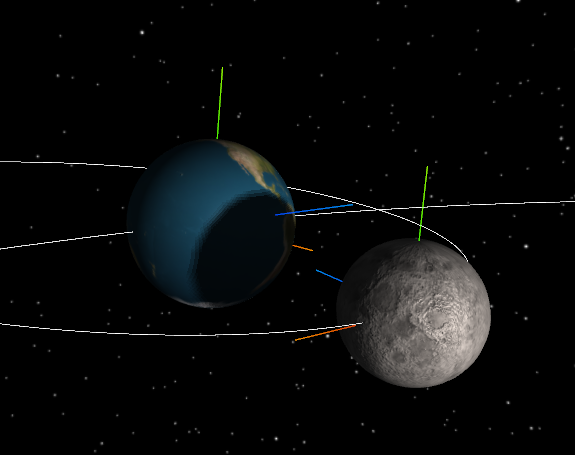
\includegraphics[width=\textwidth]{images/eclipse1}
                \caption{The Moon casting its shadow on the Earth's surface.}
                \label{fig: The Moon casting its shadow on the Earth's surface.}
	 \end{subfigure}
        \begin{subfigure}[b]{0.4\textwidth}
                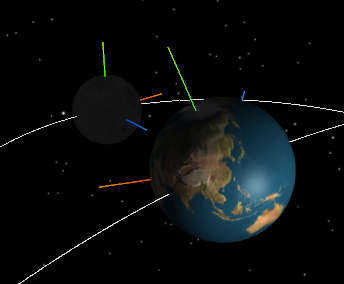
\includegraphics[width=\textwidth]{images/eclipse2}
                \caption{The Earth casting its shadow on the Moon's surface.}
                \label{fig:The Earth casting its shadow on the Moon's surface.}
	 \end{subfigure}
	 \caption{The Earth and Moon casting their shadows on each other, which can result in an eclipse of the Sun.}
\end{figure}

To get this effect is very simple, as just a couple of flags need to be set for the objects that need to be affected by this. There must be the correct materials (Lambert and Phong) and lighting (Spot, Directional - Although as of writing this, I believe PointLight either works now or a solution is being worked on) in order for this effect to work.
\begin{lstlisting}
  renderer.shadowMap.enabled = true;
  sunLight.castShadow = true;
  
  earthMesh.castShadow = true;
  earthMesh.receiveShadow = true;
  
  moonMesh.castShadow = true;
  moonMesh.receiveShadow = true;
\end{lstlisting}

In order to test that the eclipse shadows worked, I used the CameraHelper class of three.js with the shadow camera of the simulations SpotLight.
\begin{lstlisting}
sunLight = new THREE.SpotLight(0xfff0e6, 1, 0);
sunLight.castShadow = true;
sunLight.shadowCameraNear = 20;
sunLight.shadowCameraFar = 190;
sunLight.shadowCameraFov = 45;
// awesome for debugging - Shows the Shadow Camera lines
//scene.add(new THREE.CameraHelper( sunLight.shadow.camera ));
sunLight.target = earthMesh;    
sunLight.position.set(0, 0, 0);
sunMesh.add(sunLight);
\end{lstlisting}

\begin{figure}[H]
        \centering
                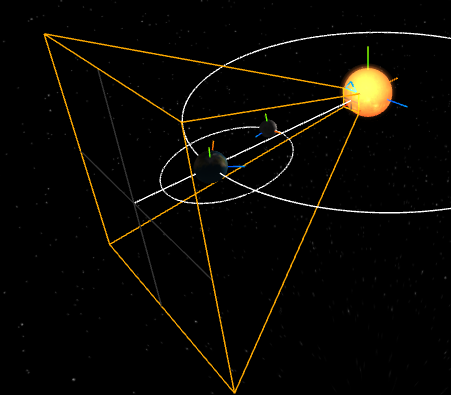
\includegraphics[width=0.5\textwidth]{images/shadowcamera}
                \caption{The Sun light Shadow Camera, showing where shadow casting will be computed.}
                \label{fig: The Shadow Camera.}
\end{figure}

You can see the ShadowCamera of the SpotLight in figure 18, as displayed by the ShadowCameraHelper. This helper shows us what the catchment area of the cast shadows will be. Computing where shadows should fall is expensive, and so I've made the shadow camera area small, in order to reduce the cost of computation.

When I first enabled the casting and receiving of shadows I encountered issues with double shadows, where a shadow would be shown on the correct side of the object shadowed but also on the reverse side. I struggled with the problem for a long time, trying to debug where I had gone wrong within my code to cause this effect. I wasn't sure if I had slightly transparent objects, if there was an issue recalculating the face and vertex normals or if I had set up my shadow camera incorrectly. In the end, it turned out that it was something I couldn't do anything about, as it was a WebGL issue\cite{shadow1}\cite{shadow2} within three.js that was only fixed a couple of weeks after the version of three.js I was using was downloaded for my application. Updating to the latest version of three.js fixed this issue!

\subsection{Other features of my choice}
As an addition to the previously mentioned features, I also wanted to implement something we'd discussed in lectures. The most obvious choice for this was matrix transformations. I implemented a number of different transformations for shifts and rotations, and started my project with using them to compute orbit. After I moved to precomputing the orbital rotations for Elliptical orbits and using Kepler's 2nd Law, the matrix transformations are now just used for the axial rotations of each object and the initial setup for the tilt of the Moon's orbit.

I came across a number of problems when I first started using matrices, and while I don't have screenshots to display some of the strange graphical errors encountered, I have described the most notable below:
\begin{itemize}
 \item The Earth gradually shrank into a cylinder - Caused by an incorrect rotation matrix that wasn't applying the `w' coordinate properly after a shift and rotation.
 \item The Earth and Moon not being captured in the Sun's gravitational pull - Caused by the way my matrices were multiplied being completely incorrect, as the way that coordinates are stored in three.js are not the same as I was expecting when I first wrote my matrix multiplication method. This also caused some issues where the Earth would become a mess of pixels.
 \item The lighting of the Earth and Moon staying in a constant position, even as the Earth and Moon rotated on their axis and moved around on their orbital rotation, the direction of the light would stay where it was when the simulation first started. - Caused by not correctly re-calculating the face and vertex normals after a matrix transformation.
 \item The vertices correctly updating after a matrix transformation but no actual difference being rendered - Caused by too much computation on each render step and creating too many new Vector3 objects. This got the system stuck in updating the data of the objects, but the renderer still waiting and not updating the objects after transformation.
\end{itemize}

There were many other smaller issues along the way, and multiple different ways of attempting to apply my own matrices to the objects, but in the end the method that works the best for me is to:
\begin{itemize}
\item After initialization, get the physical coordinates of the vertices of the objects and hold them in memory
\item Turn the coordinates into homogeneous coordinates
\item During every run step, multiple the homogeneous coordinates with the next transformation matrix for this step
\item Turn the homogeneous coordinates into physical coordinates, keeping the updated homogeneous coordinates in memory
\item Update the object with the new vertices
\item Update the face and vertex normals with the normal of the transformation matrix
\item Set flags on the object that it has been updated and needs to be rendered
\end{itemize}

In code using the Earth as an example, this looks somewhat like this (this is extracted from multiple methods in order to be demonstrated here):

\begin{lstlisting}
// initiate - Get homogeneous coordinates in memory
computableEarthVertices = convertPhysicalToHomogeneous(earthMesh.geometry.vertices);

function convertPhysicalToHomogeneous(coordinateArray){
    var result = rearrangeVertices(coordinateArray);
    result[3] = [];
    for(var i=0; i < result[0].length; i++){
        result[3][i] = 1;
    }
    return result;
}

function rearrangeVertices(coordinateArray){
    var result = [];
    for(var x = 0; x < 3; x++){
        result[x] = [];    
        for(var y = 0; y < coordinateArray.length; y++){ 
            result[x][y] = 0;
        }  
    } 
    for(var i=0; i < coordinateArray.length; i++){
        result[0][i] = coordinateArray[i].x;
    }
    for(var i=0; i < coordinateArray.length; i++){
        result[1][i] = coordinateArray[i].y;
    }
    for(var i=0; i < coordinateArray.length; i++){
        result[2][i] = coordinateArray[i].z;
    }
    return result;
}
\end{lstlisting}
\begin{lstlisting}
// update the computable vertices (homogeneous) and apply it to the object
// Once per animation frame
computableEarthVertices = updateYRotation(controlValues.earthAxisRotationSpeed * (Math.PI / 180), earthMesh.geometry, computableEarthVertices);

function updateYRotation(rotation, geometry, computableVertices){
    computableVertices = multiplyMatrices(rotationYTransformation(rotation), computableVertices);
    applyHomogeneousToPhysical(computableVertices, geometry.vertices);
    var normalMatrix = tempMatrix3.getNormalMatrix(rotationYMatrix4(rotation));
    updateFaceAndVertexNormals(normalMatrix, geometry);
    geometry.verticesNeedUpdate = true;
    geometry.normalsNeedUpdate = true;

    return computableVertices;
}

function multiplyMatrices(matrixOne, matrixTwo){
    if(matrixOne[0].length != matrixTwo.length){
        alert("MatrixOne columns do not match MatrixTwo rows. Cannot compute!");
    } else {
        var result = [];
    for(var x = 0; x < matrixOne.length; x++){
        result[x] = [];    
        for(var y = 0; y < matrixTwo[0].length; y++){ 
            result[x][y] = 0;    
        }    
    }

    for(var r=0; r < matrixTwo.length; r++){
        for(var c=0; c < matrixTwo[0].length; c++){
            for(var i=0; i < matrixOne[0].length; i++){
                result[r][c] += (matrixOne[r][i] * matrixTwo[i][c]);
            }
        }
    }

    return result;
    }
}

var rotationYTransformation = function (angle) {
    return [
        [Math.cos(angle), 0, Math.sin(angle), 0],
        [0,1,0,0],
        [-Math.sin(angle), 0, Math.cos(angle), 0],
        [0,0,0,1]
    ]; 
}

var rotationYMatrix4 = function (angle) {     
        tempMatrix4.set(
            Math.cos(angle), 0, Math.sin(angle), 0,
            0,1,0,0,
            -Math.sin(angle), 0, Math.cos(angle), 0,
            0,0,0,1
            );
        
        return tempMatrix4;
}

function applyHomogeneousToPhysical(homogeneous, physical){
    for(var x = 0; x < homogeneous[0].length; x++){
        physical[x].setX(homogeneous[0][x] / homogeneous[3][x]);
        physical[x].setY(homogeneous[1][x] / homogeneous[3][x]);
        physical[x].setZ(homogeneous[2][x] / homogeneous[3][x]); 
    }
}

function updateFaceAndVertexNormals(normalMatrix, geometry){
    for ( var i = 0, il = geometry.faces.length; i < il; i ++ ) {
        var face = geometry.faces[ i ];
        face.normal.applyMatrix3( normalMatrix ).normalize();
        for ( var j = 0, jl = face.vertexNormals.length; j < jl; j ++ ) {
            face.vertexNormals[ j ].applyMatrix3( normalMatrix ).normalize();
        }
    }

    if ( geometry.boundingBox !== null ) {
        geometry.computeBoundingBox();
    }
    if ( geometry.boundingSphere !== null ) {
        geometry.computeBoundingSphere();
    }
}
\end{lstlisting}

While this may not be the most efficient way, it was how I found I was able to extract the data from the WebGL/three.js objects, modify it and then put it back in using my own code, to show that this is something I am capable of doing and have greater control over the objects.

I am aware that there are better methods of applying matrices provided by three.js, and that for just rotation matrices I could also remove the step of converting to and from homogeneous coordinates. However, for the sake of the simulation, the potential for expansion in the future and my own challenge, I have kept the process this way.

As a final additional step, I added a star map to surround the simulation, to help the user navigate around the scene easier and give a tiny bit more visual interest and realism. The inspiration for this came from `learningthreejs'\cite{learningthreejs}. The star map texture is from Paul Bourke\cite{startexture}.

\begin{figure}[H]
        \centering
                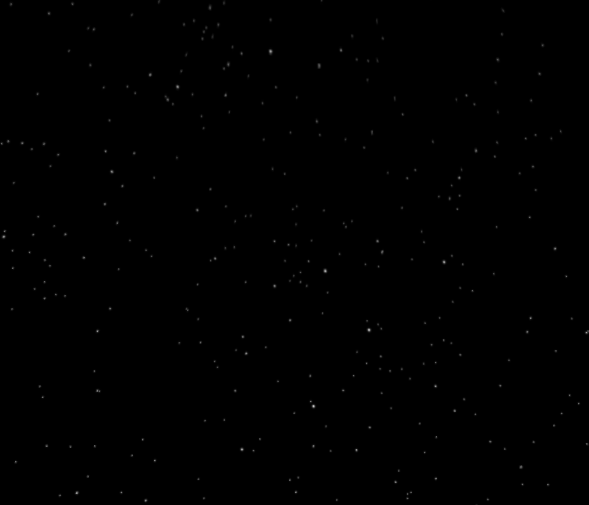
\includegraphics[width=0.5\textwidth]{images/stars}
                \caption{A portion of the star texture map.}
                \label{fig: Star map.} 
\end{figure}

\begin{lstlisting}
// Simple sphere that surrounds the simulation, to give the appearance that all takes place within the universe and the camera can move around it.
function buildStarMapMesh(){
  var starGeometry  = new THREE.SphereGeometry(starMapSize, 32, 32);
  var starTexture = textures.starMap;
  starTexture.wrapS = starTexture.wrapT = THREE.RepeatWrapping; 
  var starMaterial = new THREE.MeshBasicMaterial( {map: starTexture } );
  starMaterial.side = THREE.BackSide;
  var starMesh = new THREE.Mesh(starGeometry, starMaterial);
  return starMesh;
}
\end{lstlisting}
%----------------------------------------------------------------------------------------
%	SELF ASSESSMENT
%----------------------------------------------------------------------------------------

\section{Self Assessment}
\begin{tabular}{ | l | l | l | c | r | r | r |}
\hline	
Task &  documented & implemented &  & Extension & documented & implemented \\
\hline
1 & \checkmark & \checkmark & & a) &\checkmark  &\checkmark  \\
 \hline
2 & \checkmark & \checkmark & & b) & \checkmark &\checkmark  \\
 \hline
3 & \checkmark & \checkmark & & c) & \checkmark &\checkmark  \\
 \hline
4 &\checkmark  & \checkmark & & d) & \checkmark &\checkmark  \\
 \hline
5 &\checkmark  &\checkmark  & & e) & \checkmark &\checkmark  \\
 \hline
6 & \checkmark & \checkmark & & f) & \checkmark &\checkmark  \\
 \hline
7 & \checkmark &\checkmark  & & g) &\checkmark  &\checkmark  \\
 \hline
 & & & & h) &\checkmark  &\checkmark  \\
  \hline
 & & & & i) &\checkmark  &\checkmark  \\
  \hline
 & & & & j) &\checkmark  &\checkmark  \\
 \hline
 \multicolumn{6}{|l|}{Animation can be viewed in B57, C56 without additional software} & \checkmark \\
  \hline
  \multicolumn{6}{|l|}{All reference sources are acknowledged} & \checkmark \\
 \hline	
 \multicolumn{7}{l}{Your overall self-assessment out of 50:    \textbf{47/50}}
\end{tabular}


From implementing all of the basic features as requested and then all of the additional features, I feel my grade for those sections should be high. I have a feeling that my report may bring my mark down slightly, due to my style of writing and my tests being mainly visual rather than data tables, and that it is very long in length. Through this, I would award myself the mark shown above.

%----------------------------------------------------------------------------------------
\clearpage

%----------------------------------------------------------------------------------------
%	REFERENCES
%----------------------------------------------------------------------------------------

\begin{thebibliography}{5}

\bibitem{assignment} H. Holstein and Y. Liu, ``A virtual Sun-Earth-Moon system'', CS32310 Advanced Computer Graphics Assignment Semester 1 2015, October 14 2015

\bibitem{xampp} ApacheFriends.org, {\em `XAMPP Installers and Downloads for Apache Friends' }, [online], 
Available: https://www.apachefriends.org/index.html [Accessed 11/06/2015]

\bibitem{earthtextures} PlanetPixelEmporium.com, {\em `Planet Texture Map Collection'}, [online],
Available: http://planetpixelemporium.com/planets.html [Accessed 11/06/2015]

\bibitem{suntexture} NASA.gov, {\em `NASA'}, [online], Available: 

https://www.nasa.gov/sites/default/files/images/700328main\_20121014\_003615\_flat.jpg [Accessed 11/06/2015]

\bibitem{sunglow} Stemkoski.Blogspot.co.uk, {\em `Computational Contemplations: Using Shaders and Selective Glow Effects in Three.js'}, [online],
Available: http://stemkoski.blogspot.co.uk/2013/03/using-shaders-and-selective-glow.html [Accessed 11/06/2015]

\bibitem{datgui}, GitHub.com {\em `three.js/dat.gui.min.js at master . mrdoob/three.js'}, [online],
Available: https://github.com/mrdoob/three.js/blob/master/examples/js/libs/dat.gui.min.js [Accessed 11/06/2015]

\bibitem{orbitcontrols} GitHub.com {\em `three.js/OrbitControls.js at master . mrdoob/three.js'}, [online],
Available: https://github.com/mrdoob/three.js/blob/master/examples/js/controls/OrbitControls.js [Accessed 11/06/2015]

\bibitem{shadow1} StackOverflow.com, {\em `webgl - THREE.JS Shadow on opposite side of light - Stack Overflow'}, [online],
Available: http://stackoverflow.com/a/12602143 [Accessed 11/07/2015]

\bibitem{shadow2} StackOverflow.com, {\em `Three.js DoubleSided material doesn't cast shadow on both sides of planar parametric geometry'}, [online],
Available: http://stackoverflow.com/a/20473174 [Accessed 11/07/2015]

\bibitem{learningthreejs} LearningThreeJS.com, {\em `How To Make The Earth In WebGL? - Learning Three.js'}, [online],
Available: http://learningthreejs.com/blog/2013/09/16/how-to-make-the-earth-in-webgl/ [Accessed 11/07/2015]

\bibitem{startexture} PaulBourke.net, {\em `Representing star fields'}, [online],
Available: http://paulbourke.net/miscellaneous/starfield/ [Accessed 11/07/2015]

\bibitem{codecolour}  Acknowledgement for code colouring in this report using lstlisting LaTeX: 

TeX.StackExchange.com, {\em `javascript - language option supported in listings - TeX - LaTeX Stack Exchange'}, [online],

Available: http://tex.stackexchange.com/questions/89574/language-option-supported-in-listings [Accessed: 11/06/2015]

\end{thebibliography}


\end{document}


